\chapter{ĐÁNH GIÁ}
\label{chap:5-evaluation}

% TODO: đoạn dẫn nhập chương

\section{Thiết lập thực nghiệm}
\label{sec:5-setup}

Mọi kết quả trong chương này được đo trên cùng một môi trường. Mỗi bảng kết quả ở các mục sau chỉ ghi các tham số khác với mục này.

\subsection{Phần cứng và phần mềm}
\label{sec:5-hardware}

{\small
\begin{longtblr}[
  caption = {Môi trường thực nghiệm},
  label = {tab:5-environment},
]{
  width = \linewidth,
  rowhead = 1,
  colspec = {X[1.4,l]X[3,l]}, rows = {abovesep=2pt, belowsep=2pt},
  hlines, vlines, row{1} = {font=\bfseries, bg=gray!20},
}
Hạng mục & Giá trị \\
CPU & Apple M5, 10 nhân (4 nhân hiệu năng, 6 nhân tiết kiệm), kiến trúc ARM64 \\
RAM của máy & 24~GB \\
Bộ nhớ cấp cho Docker & 11,7~GiB (OrbStack 2.2.5) \\
Ổ đĩa & SSD 926~GiB, còn trống khoảng 716~GiB \\
Hệ điều hành & macOS 27.2.1 \\
Docker Engine, Compose & Docker Engine 29.8.2, Compose 5.5.0 \\
Thành phần hệ thống & Theo Bảng~\ref{tab:4-versions} \\
Spark & \code{local[*]}, driver 2~GB, 4 nhân, 4 phân vùng shuffle \\
\end{longtblr}
}

\subsection{Dữ liệu thực nghiệm}
\label{sec:5-data}

Dữ liệu được sinh bởi bộ mô phỏng cảm biến (Mục~\ref{sec:4-application}) dựa trên dữ liệu danh mục \code{reference/reference\_data.json}: 4 trang trại, 8 thửa ruộng, 24 thiết bị, 4 loại cây trồng (lúa, ngô, cà chua, cà phê) và 5 chỉ số. Mỗi thiết bị báo cáo 5 giây một lần. Các giá trị ngẫu nhiên của bộ mô phỏng có hạt giống cố định, nhưng thời điểm đo lấy từ đồng hồ thật và mã sự kiện là UUID ngẫu nhiên, nên hai lần chạy cho chuỗi sự kiện tương tự chứ không giống hệt; vì vậy các kiểm tra ở Mục~\ref{sec:5-correctness} so với nhãn đi kèm từng sự kiện chứ không so với một tập dữ liệu cố định.

Bộ mô phỏng tiêm lỗi có chủ đích và đánh dấu mỗi sự kiện lỗi bằng trường \code{simulated\_fault}. Trường này đi theo bản ghi vào bronze (và nằm trong \code{raw\_payload} của bản ghi bị cách ly), nên có thể so số lỗi tiêm vào với số lỗi hệ thống phát hiện được mà không cần nhãn bên ngoài.

{\small
\begin{longtblr}[
  caption = {Cấu hình bộ mô phỏng (\texttt{.env.example})},
  label = {tab:5-simulator},
]{
  width = \linewidth,
  rowhead = 1,
  colspec = {X[1.8,l]X[1.2,l]X[2.6,l]}, rows = {abovesep=2pt, belowsep=2pt},
  hlines, vlines, row{1} = {font=\bfseries, bg=gray!20},
}
Tham số & Mặc định & Ý nghĩa \\
\code{SIM\_SEED} & 42 & Hạt giống ngẫu nhiên \\
\code{SIM\_RATE\_HZ} & 1 & Số nhịp sinh dữ liệu mỗi giây \\
\code{SIM\_FAULT\_RATE} & 0,05 & Xác suất ở mỗi nhịp có một thiết bị ngẫu nhiên được lên lịch tiêm lỗi \\
\code{SIM\_FAULTS} & 7 loại & \code{null\_value}, \code{out\_of\_range}, \code{implausible\_jump}, \code{duplicate}, \code{unknown\_device}, \code{unexpected\_metric}, \code{malformed} \\
\code{SIM\_GAP\_RATE} & 0,002 & Xác suất ở mỗi nhịp có một thiết bị ngẫu nhiên bắt đầu im lặng \\
\code{SIM\_GAP\_SECONDS\_MIN/MAX} & 45 / 90 & Độ dài khoảng im lặng (giây) \\
\code{SIM\_DURATION\_SECONDS} & 0 & Thời gian chạy một lần thực nghiệm (0 = chạy liên tục; mỗi benchmark tự bật, tắt bộ mô phỏng và ghi độ dài cửa sổ đo vào CSV) \\
\end{tblr}
\end{table}

\subsection{Tham số của đường xử lý}
\label{sec:5-params}

{\small
\begin{longtblr}[
  caption = {Tham số mặc định của tác vụ streaming và cảnh báo},
  label = {tab:5-params},
]{
  width = \linewidth,
  rowhead = 1,
  colspec = {X[2,l]X[1,l]X[2.6,l]}, rows = {abovesep=2pt, belowsep=2pt},
  hlines, vlines, row{1} = {font=\bfseries, bg=gray!20},
}
Tham số & Giá trị & Ý nghĩa \\
\code{TRIGGER\_INTERVAL} & 30 s & Chu kỳ micro-batch (benchmark \#1 đổi thành 10 s và 60 s) \\
\code{MAX\_OFFSETS\_PER\_TRIGGER} & 20\,000 & Số sự kiện tối đa mỗi lô \\
\code{WATERMARK\_S} & 3\,600 & Cửa sổ chấp nhận dữ liệu đến muộn \\
\code{LATE\_AFTER\_S} & 600 & Ngưỡng gắn cờ \code{is\_late} \\
\code{ALERT\_DEBOUNCE\_BATCHES} & 2 & Số lô vi phạm liên tiếp trước khi cảnh báo \\
\code{ALERT\_COOLDOWN\_S} & 300 & Khoảng tối thiểu giữa hai cảnh báo cùng điều kiện \\
\code{DEVICE\_OFFLINE\_MULTIPLIER} & 4 & Im lặng quá 4 lần chu kỳ báo cáo (20 s) thì coi là mất kết nối \\
\code{BATTERY\_LOW\_PCT} & 20 & Ngưỡng pin yếu (\%) \\
\code{SIGNAL\_POOR\_MAX} & 0,3 & Ngưỡng sóng yếu \\
\end{longtblr}
}

\subsection{Quy trình chạy lại}
\label{sec:5-procedure}

Các benchmark chạy trên tập dữ liệu tích lũy của hệ thống (khoảng 41 nghìn số đo trong bronze trên 12 ngày có dữ liệu, cộng dữ liệu sinh ra trong lúc đo), không xóa sạch giữa các lần đo, vì một số phép đo (gold, time travel, compaction) cần lịch sử. Benchmark \#2--\#4 tự tạo dữ liệu tổng hợp của mình trong schema \code{bench}. Trình tự đã dùng:

\begin{lstlisting}[language=bash, caption={Trình tự chạy các benchmark và kiểm tra}, label={lst:5-procedure}]
just up && just up-app        # all profiles, data volumes kept
just bench-lookups            # #2  (stream and simulator stopped)
just bench-storage            # #3
just bench-compaction         # #4
just bench-trigger            # #1  restarts spark-stream per interval
just bench-replay             # #5  kills/stops spark-stream, checks Kafka vs bronze
just stop-stream && just batch-run   # dbt + tests + compaction (bronze, ops)
just check-correctness --since <time of the simulator fix>   # section 5.2
just run-stream-bg && just bench-web   # #6 (stream and simulator running)
\end{lstlisting}

Kết quả của từng benchmark được lưu trong \code{benchmarks/results/*.csv}, với cấu hình của lần đo (máy, phiên bản, tải, cửa sổ đo, trigger) ghi ở các dòng đầu tệp.

\section{Tính đúng đắn của dữ liệu}
\label{sec:5-correctness}

Mục này kiểm tra dữ liệu sau khi qua đường xử lý có đúng hay không, theo bốn câu hỏi:

\begin{enumerate}
  \item Mọi lỗi được tiêm vào có bị phát hiện và đếm đúng không?
  \item Tầng gold có khớp với tầng silver không?
  \item Tầng gold có chứa giá trị phi lý không?
  \item Sau khi tác vụ bị dừng và khởi động lại, có mất hoặc trùng dữ liệu không?
\end{enumerate}

Mọi lần đo dùng môi trường và quy trình ở Mục~\ref{sec:5-setup}.

\subsection{Phát hiện lỗi được tiêm vào}
\label{sec:5-fault-detection}

\paragraph{Phương pháp.} Bộ mô phỏng gắn nhãn \code{simulated\_fault} cho mỗi sự kiện lỗi. Mỗi loại lỗi có một kết quả mong đợi: hoặc bị cách ly với một lý do cụ thể, hoặc được giữ lại với một cờ chất lượng cụ thể (Bảng~\ref{tab:5-fault-expect}). Script \code{benchmarks/run\_correctness\_checks.py} (\code{just check-correctness}) lấy Kafka làm nguồn sự thật: nó đọc lại mọi thông điệp trong khoảng thời gian kiểm tra, đếm số sự kiện tiêm vào theo nhãn, rồi tìm nơi mỗi nhãn kết thúc trong bronze (với cờ nào) và trong \code{ops.quarantine} (với lý do nào), lọc theo đúng các offset đó. Một sự kiện được tính là \emph{phát hiện} khi nó không đi vào dữ liệu sạch (bị gắn cờ khác \code{ok} hoặc bị cách ly), và \emph{phân loại đúng} khi cờ hoặc lý do khớp Bảng~\ref{tab:5-fault-expect}.

\begin{table}[H]
\centering
\caption{Kết quả mong đợi cho từng loại lỗi được tiêm vào}
\label{tab:5-fault-expect}
\small
\begin{tblr}{
  colspec = {X[1.6,l]X[2.8,l]X[2,l]}, rows = {abovesep=2pt, belowsep=2pt},
  hlines, vlines, row{1} = {font=\bfseries, bg=gray!20},
}
Lỗi tiêm vào & Cách bộ mô phỏng tạo lỗi & Kết quả mong đợi \\
\code{null\_value} & Giá trị đo là \code{null} & Cờ \code{null\_value} \\
\code{out\_of\_range} & Giá trị lớn hơn ngưỡng tối đa từ 5 đến 50 đơn vị & Cờ \code{out\_of\_range} \\
\code{implausible\_jump} & Giá trị lệch 2--3 lần bước nhảy tối đa, vẫn trong khoảng vật lý & Cờ \code{implausible\_jump} \\
\code{duplicate} & Gửi lại nguyên một payload đã gửi trước đó & Cờ \code{duplicate}, chỉ một bản vào bronze \\
\code{unknown\_device} & Mã thiết bị không có trong danh mục & Cách ly, lý do \code{unknown\_device} \\
\code{unexpected\_metric} & Tên chỉ số sai (\code{\ldots\_typo}) & Cách ly, lý do \code{unexpected\_metric} \\
\code{malformed} & Thiếu trường, thời gian sai, giá trị không phải số & Cách ly, lý do \code{missing\_field}, \code{invalid\_timestamp} hoặc \code{malformed\_value} \\
\end{tblr}
\end{table}

Có ba điểm cần lưu ý khi đếm:

\begin{itemize}
  \item \textbf{Đếm bản sao.} Với lỗi \code{duplicate}, bộ mô phỏng giữ payload ở lần đầu thiết bị bị chọn và chỉ gửi lại ở lần thứ hai. Số bản sao thật vì vậy phải đếm bằng số \code{event\_id} lặp lại, không đếm bằng số nhãn.
  \item \textbf{Bản sao đến ở lô khác.} Cờ \code{duplicate} được gán bằng \code{row\_number()} \emph{trong một lô}. Nếu bản sao đến ở một lô sau, nó mang cờ \code{ok} và lệnh \code{MERGE} gộp nó vào dòng đã có. Bronze vẫn không bị trùng, nhưng bảng đếm sẽ ghi thiếu số bản sao. Đây là nguồn lệch có thể có của dòng \code{duplicate} trong Bảng~\ref{tab:5-fault-result}.
  \item \textbf{Bước nhảy.} Bước nhảy được so với giá trị mới nhất của cả thửa ruộng, nên một giá trị bước nhảy đến ngay sau một giá trị ngoài khoảng có thể không bị coi là bước nhảy.
\end{itemize}

Câu truy vấn~\ref{lst:5-fault-count} đếm cả hai phía trên Trino.

\begin{lstlisting}[language=SQL, caption={Đếm lỗi tiêm vào và lỗi phát hiện trên Trino}, label={lst:5-fault-count}]
-- Faults kept in bronze: injected label vs quality flag
SELECT simulated_fault, quality_flag, count(*) AS n
FROM lakehouse.bronze.sensor_readings
WHERE simulated_fault IS NOT NULL
GROUP BY 1, 2 ORDER BY 1, 2;

-- Faults sent to quarantine: injected label (from the raw payload) vs reason
SELECT json_extract_scalar(raw_payload, '$.simulated_fault') AS injected,
       reason, count(*) AS n
FROM lakehouse.ops.quarantine
GROUP BY 1, 2 ORDER BY 1, 2;

-- Duplicates removed before bronze
SELECT sum(duplicate) FROM lakehouse.ops.quality_counters;
\end{lstlisting}

\paragraph{Kết quả.} Bảng~\ref{tab:5-fault-result} là kết quả trên mọi thông điệp gửi từ 17:23 UTC ngày 12/11/2026 tới khi kết thúc các benchmark (51\,755 thông điệp, khoảng 2,5 giờ chạy với tỷ lệ lỗi mặc định, \texttt{benchmarks/results/correctness.csv}). Cột cuối là lần kiểm tra đầu tiên, chạy trên toàn bộ dữ liệu Kafka còn giữ \emph{trước khi} sửa bộ mô phỏng (xem phần nhận xét).

\begin{table}[H]
\centering
\caption{Lỗi tiêm vào, lỗi phát hiện và lỗi được phân loại đúng}
\label{tab:5-fault-result}
\small
\begin{tblr}{
  colspec = {X[1.9,l]X[0.9,c]X[0.9,c]X[1.1,c]X[1.6,c]}, rows = {abovesep=2pt, belowsep=2pt},
  hlines, vlines, row{1} = {font=\bfseries, bg=gray!20},
}
Loại lỗi & Tiêm vào & Phát hiện & Phân loại đúng & Trước khi sửa (đúng / tiêm) \\
\code{null\_value} & 80 & 80 & 80 & 52 / 52 \\
\code{out\_of\_range} & 105 & 105 & 105 & 57 / 57 \\
\code{implausible\_jump} & 72 & 72 & 72 & 2 / 92 \\
\code{unknown\_device} & 103 & 103 & 103 & 67 / 67 \\
\code{unexpected\_metric} & 72 & 72 & 72 & 83 / 83 \\
\code{malformed} & 121 & 121 & 121 & 61 / 78 \\
\code{duplicate} (bản gửi lại) & 48 & 48 & 48 & 18 / 18 \\
\textbf{Tổng} & \textbf{601} & \textbf{601} & \textbf{601 (100\,\%)} & 340 / 447 \\
\end{tblr}
\end{table}

Sau khi sửa, mọi lỗi được tiêm vào đều bị phát hiện và phân loại đúng. Với lỗi \code{duplicate}, 48 bản gửi lại không tạo thêm dòng nào trong bronze (số dòng trừ số \code{event\_id} khác nhau bằng 0), và \code{ops.quality\_counters} đếm đúng 48 bản trùng: trong lần chạy này các bản gửi lại đều đến đủ sớm để được phát hiện, nên nguồn lệch dự đoán ở trên không xảy ra.

\paragraph{Ba lỗi của bộ mô phỏng do kiểm tra này phát hiện.} Lần kiểm tra đầu cho kết quả khác, và cả ba chỗ lệch đều nằm ở bộ mô phỏng chứ không ở đường xử lý:

\begin{enumerate}
  \item \textbf{Bước nhảy vượt khoảng vật lý.} Bộ mô phỏng tạo bước nhảy bằng 3--10 lần bước nhảy tối đa, nên giá trị gần như luôn vượt khoảng của chỉ số; vì kiểm tra khoảng chạy trước, 90/92 lỗi bị gắn cờ \code{out\_of\_range} thay vì \code{implausible\_jump}. Dữ liệu vẫn bị loại khỏi dữ liệu sạch, nhưng kiểm tra bước nhảy gần như không được thử. Bộ mô phỏng được sửa để tạo bước nhảy 2--3 lần, giữ trong khoảng vật lý.
  \item \textbf{Biến thể ``JSON hỏng'' không hỏng.} Biến thể này chỉ thêm một khóa lạ vào payload; cổng HTTP chỉ nhận đối tượng JSON và tuần tự hóa lại, nên thông điệp tới Kafka luôn là JSON hợp lệ và được giữ với cờ \code{ok} (17 sự kiện), đúng theo schema tường minh. Biến thể bị bỏ; JSON hỏng thật sự bị cổng HTTP từ chối với mã 422 và không bao giờ tới Kafka.
  \item \textbf{Giá trị bình thường ra ngoài khoảng.} Nhiễu đo được cộng \emph{sau} bước giới hạn khoảng, nên 643 số đo không mang nhãn lỗi nằm ngoài khoảng (lượng mưa âm tới $-0{,}32$~mm/h, độ ẩm không khí tới 102\,\%). Đường xử lý đã gắn cờ đúng cả 643, nhưng chúng làm sai số liệu ``lỗi tiêm vào''. Bộ mô phỏng được sửa để giới hạn cả giá trị cuối cùng; sau khi sửa, 0 số đo không mang nhãn bị gắn cờ \code{out\_of\_range}.
\end{enumerate}

Mỗi lỗi có một kiểm thử đơn vị trong \code{tests/unit/test\_simulator.py}; kiểm thử về khoảng giá trị thất bại trên mã cũ và đạt trên mã mới.

\paragraph{Cảnh báo giả của kiểm tra bước nhảy.} 86 trong 51\,080 số đo lành mạnh (0,17\,\%) bị gắn cờ \code{implausible\_jump}. 80 trong số đó đứng ngay sau một số đo khác của cùng thửa ruộng và chỉ số đã bị gắn cờ \code{implausible\_jump}: giá trị mới nhất trong \code{latest\_by\_field}, dùng làm mốc so bước nhảy, nhận cả các số đo có cờ \code{implausible\_jump} (để bảng điều khiển hiển thị chúng kèm cờ), nên sau một giá trị bất thường, số đo bình thường kế tiếp bị so với giá trị bất thường đó. Đây là một hạn chế của đường xử lý được ghi nhận lại; cách sửa là chỉ lấy số đo \code{ok} cuối cùng làm mốc so bước nhảy.

\subsection{Đối soát tầng gold với tầng silver}
\label{sec:5-reconciliation}

\paragraph{Phương pháp.} Không lấy mẫu: \emph{mọi} dòng của \code{gold.field\_daily} được tính lại trực tiếp từ silver theo đúng định nghĩa của model (min, max, trung bình chỉ trên dòng \code{quality\_flag = 'ok'}; \code{reading\_count} trên mọi giá trị khác rỗng; \code{valid\_count} trên dòng \code{ok}) rồi so sánh. Truy vấn~\ref{lst:5-reconcile} đếm các dòng lệch; truy vấn thứ hai đếm các bộ (thửa ruộng, chỉ số, ngày) có trong silver mà thiếu trong gold. Kết quả mong đợi của cả hai là 0.

\begin{lstlisting}[language=SQL, caption={Đối soát gold với silver trên Trino (rút gọn từ \texttt{run\_correctness\_checks.py})}, label={lst:5-reconcile}]
WITH recomputed AS (
    SELECT field_id, metric, CAST(date_trunc('day', measured_at) AS date) AS day,
           min(CASE WHEN quality_flag = 'ok' THEN value END) AS min_value,
           max(CASE WHEN quality_flag = 'ok' THEN value END) AS max_value,
           avg(CASE WHEN quality_flag = 'ok' THEN value END) AS avg_value,
           count(*) AS reading_count,
           count_if(quality_flag = 'ok') AS valid_count
    FROM lakehouse.silver.sensor_readings
    WHERE value IS NOT NULL
    GROUP BY 1, 2, 3
)
SELECT count(*) AS compared,
       count_if(r.day IS NULL
                OR g.reading_count <> r.reading_count
                OR g.valid_count <> r.valid_count
                OR g.min_value IS DISTINCT FROM r.min_value
                OR g.max_value IS DISTINCT FROM r.max_value
                OR abs(g.avg_value - r.avg_value) > 1e-9) AS mismatched
FROM lakehouse.gold.field_daily g
LEFT JOIN recomputed r
  ON g.field_id = r.field_id AND g.metric = r.metric AND g.day = r.day;
\end{lstlisting}

\paragraph{Kết quả.} Sau \code{just batch-run}, 520/520 dòng của \code{gold.field\_daily} khớp với giá trị tính lại từ silver (0 dòng lệch về số đếm, min, max hay trung bình), và 0 bộ (thửa ruộng, chỉ số, ngày) của silver bị thiếu trong gold. Mục~\ref{sec:4-br06} dùng cùng cách tính lại để kiểm tra trung bình có trọng số của trang so sánh giai đoạn.

\subsection{Giá trị phi lý trong tầng gold}
\label{sec:5-implausible}

\paragraph{Phương pháp.} Đếm số dòng của \code{gold.field\_daily} có \code{min\_value} hoặc \code{max\_value} nằm ngoài khoảng vật lý \emph{riêng của từng chỉ số} (Bảng~\ref{tab:4-metric-ranges}), chặt hơn test \code{accepted\_range} chung $[-30, 200]$ của dbt.

\paragraph{Kết quả.} 0/520 dòng của \code{gold.field\_daily} có min hoặc max nằm ngoài khoảng của chỉ số, dù silver vẫn giữ 1\,071 số đo \code{out\_of\_range} (silver giữ mọi số đo kèm cờ, theo FR4.6). Model đã được giới hạn ở \code{quality\_flag = 'ok'} (Mục~\ref{sec:4-br04}), và \code{just dbt-test} đạt 28/28 test, gồm các test \code{accepted\_range} của gold.

\subsection{Không mất, không trùng khi khởi động lại}
\label{sec:5-no-loss}

Kiểm tra này dùng kết quả của benchmark \#5 (Mục~\ref{sec:5-bench-replay}): giết hoặc dừng tác vụ streaming 3 phút trong khi bộ mô phỏng vẫn gửi dữ liệu, khởi động lại trên cùng checkpoint, rồi đối chiếu từng thông điệp Kafka với bronze, quarantine và Cassandra, và đếm khóa \code{(device\_id, metric, measured\_at)} trùng lặp. Cơ chế bảo đảm là checkpoint của Spark (Mục~\ref{sec:2-checkpoint}) cùng các lệnh \code{MERGE} theo khóa (Mục~\ref{sec:2-idempotent}).

\begin{lstlisting}[language=SQL, caption={Kiểm tra khóa trùng trong bronze}, label={lst:5-dup-check}]
SELECT device_id, metric, measured_at, count(*) AS n
FROM lakehouse.bronze.sensor_readings
GROUP BY 1, 2, 3 HAVING count(*) > 1;
\end{lstlisting}

\paragraph{Kết quả.} Ở cả ba kịch bản (giết tác vụ đầu lô, giết ngay sau khi lô đã commit vào bronze, dừng có trật tự), 0 thông điệp bị mất, 0 khóa trùng trong bronze, 0 offset trùng trong quarantine và 0 số đo hiển thị được bị thiếu trong Cassandra, trên tổng cộng 9\,224 thông điệp Kafka (Bảng~\ref{tab:5-bench-replay}). Truy vấn~\ref{lst:5-dup-check} chạy trên toàn bộ bronze sau cả ba kịch bản cũng trả về rỗng.

\subsection{Kiểm thử đơn vị}
\label{sec:5-unit-tests}

Ngoài các kiểm tra trên dữ liệu thật, logic quyết định được kiểm thử độc lập với Spark và Cassandra bằng \code{just test-unit}: 7 kiểm thử cho máy trạng thái cảnh báo, 11 cho logic mất kết nối và khoảng trống dữ liệu, 13 cho cấu hình, 8 cho dữ liệu danh mục, 11 cho lớp gần thời gian thực của API và 7 cho giá trị của bộ mô phỏng (thêm sau khi kiểm tra ở Mục~\ref{sec:5-fault-detection} phát hiện lỗi của bộ mô phỏng). Lần chạy cuối: 57/57 kiểm thử đạt.


\section{Hiệu năng của giải pháp}
\label{sec:5-performance}
Mục này trình bày sáu benchmark mà đề tài yêu cầu (\code{AGENTS.md}, \code{REQUIREMENTS.md} mục 7). Bảng~\ref{tab:5-bench-overview} cho biết mỗi benchmark trả lời câu hỏi nào và cho yêu cầu nghiệp vụ nào. Mọi benchmark chạy trên cùng một máy (Bảng~\ref{tab:5-environment}), là một recipe \code{just} và ghi kết quả cùng cấu hình vào \code{benchmarks/results/*.csv}.

\begin{table}[H]
\centering
\caption{Sáu benchmark của đề tài}
\label{tab:5-bench-overview}
\small
\begin{tblr}{
  colspec = {X[0.4,c]X[2.4,l]X[1.6,l]X[1,l]X[1.2,l]}, rows = {abovesep=2pt, belowsep=2pt},
  hlines, vlines, row{1} = {font=\bfseries, bg=gray!20},
}
\# & Câu hỏi & Recipe, kết quả & BR & Mục \\
1 & Chu kỳ trigger 10/30/60 s: độ trễ đầu-cuối, độ trễ cảnh báo, tải, số commit & \code{bench-trigger}, \code{trigger.csv} & BR2, BR3, BR8 & \ref{sec:5-bench-trigger} \\
2 & Cassandra và Trino cho cùng câu hỏi của bảng điều khiển & \code{bench-lookups}, \code{lookups.csv} & BR2, BR5, BR7 & \ref{sec:5-bench-lookups} \\
3 & Iceberg và Hive/Parquet & \code{bench-storage}, \code{storage.csv} & BR3, BR6 & \ref{sec:5-bench-storage} \\
4 & Hiệu quả của compaction & \code{bench-compaction}, \code{compaction.csv} & BR6 & \ref{sec:5-bench-compaction} \\
5 & Phục hồi và phát lại: không mất, không trùng & \code{bench-replay}, \code{replay.csv} & BR3, BR4 & \ref{sec:5-bench-replay} \\
6 & Độ phản hồi của API và các trang web & \code{bench-web}, \code{web.csv}, \code{web\_pages.csv} & BR1, BR7 & \ref{sec:5-bench-web} \\
\end{tblr}
\end{table}

% Benchmark #1 và #5 của Mục 5.3 (người phụ trách: Nhân). Khang chạy cả hai trên cùng máy với
% các benchmark #2--#4 để mọi số liệu của chương 5 đến từ một môi trường (Bảng tab:5-bench-config).
\subsection{Benchmark lớp xử lý luồng}
\label{sec:5-bench-stream}

Hai benchmark dưới đây đo tác vụ Spark Structured Streaming khi nó \emph{đang chạy} với bộ mô phỏng, khác với ba benchmark lớp lưu trữ đo khi luồng đã dừng. Vì phải tự khởi động lại, dừng và giết container \code{spark-stream}, hai script chạy trên máy chủ bằng \code{uv run} (\code{just bench-trigger}, \code{just bench-replay}) và truy cập Kafka, Cassandra, Trino qua cổng được công bố; mọi thứ khác (máy, phiên bản, cách ghi cấu hình vào đầu tệp CSV) giống Bảng~\ref{tab:5-bench-config}.

\subsubsection{Benchmark \#1: chu kỳ trigger 10, 30 và 60 giây}
\label{sec:5-bench-trigger}

\paragraph{Câu hỏi.} Chu kỳ trigger ảnh hưởng thế nào tới thời gian một số đo xuất hiện trên bảng điều khiển, thời gian một cảnh báo mất kết nối xuất hiện, tải của tác vụ và số commit vào lakehouse? Chu kỳ 30 giây của giải pháp chính (Mục~\ref{sec:5-params}) có hợp lý không? Đây cũng là phép đo cho phương án thay thế C (Mục~\ref{sec:4-alt-trigger}).

\paragraph{Thiết kế.} Với mỗi chu kỳ, script khởi động lại \code{spark-stream} với \code{TRIGGER\_INTERVAL} tương ứng (cùng checkpoint), chờ 180 giây cho tác vụ ổn định, rồi đo trong một cửa sổ 360 giây. Bộ mô phỏng chạy liên tục với 24 thiết bị báo cáo mỗi 5 giây (khoảng 7 sự kiện/giây) và tỷ lệ lỗi mặc định; riêng tỷ lệ im lặng được tăng lên (\code{SIM\_GAP\_RATE=0.015}, mỗi lần im lặng 180--240 giây, dài hơn mọi thời gian debounce) để có đủ sự cố mất kết nối. Các đại lượng đo:

\begin{itemize}
  \item \textbf{Độ trễ đầu-cuối} của từng số đo: thời điểm Cassandra ghi dòng (\code{writetime(value)} của \code{readings\_by\_field\_24h}) trừ thời điểm Kafka nhận sự kiện (\code{ingested\_at}). Đây là thời gian từ lúc nền tảng nhận dữ liệu tới lúc API đọc được nó, đúng đại lượng của yêu cầu phi chức năng ``hiển thị trong vòng 90 giây'' (\code{REQUIREMENTS.md}, mục 6).
  \item \textbf{Độ trễ cảnh báo mất kết nối}: thời điểm Cassandra ghi cảnh báo \code{device\_offline} trừ thời điểm thiết bị vượt ngưỡng im lặng (số đo cuối cùng cộng 20 giây), cho mọi khoảng im lặng bắt đầu trong cửa sổ.
  \item \textbf{Tải}: thời gian xử lý mỗi lô (từ log của tác vụ), tỷ lệ bận (tổng thời gian xử lý chia độ dài cửa sổ), CPU và bộ nhớ của container Spark (lấy mẫu \code{docker stats} mỗi 5 giây), số commit và số tệp mới của bảng bronze (bảng \code{\$snapshots} của Iceberg), quy ra mỗi giờ.
\end{itemize}

\begin{table}[H]
\centering
\caption{Kết quả theo chu kỳ trigger, cửa sổ đo 360 giây (\texttt{benchmarks/results/trigger.csv})}
\label{tab:5-bench-trigger}
\small
\begin{tblr}{
  colspec = {X[2.8,l]X[1,c]X[1,c]X[1,c]}, rows = {abovesep=2pt, belowsep=2pt},
  hlines, vlines, row{1} = {font=\bfseries, bg=gray!20},
}
Chỉ số & 10 s & 30 s & 60 s \\
Sự kiện trong cửa sổ (sự kiện/giây) & 2\,732 (7,6) & 2\,688 (7,5) & 2\,499 (6,9) \\
Số lô / sự kiện mỗi lô (p50) & 35 / 76 & 12 / 222 & 6 / 417 \\
Thời gian xử lý một lô, p50 / p95 (s) & 6,3 / 8,4 & 7,5 / 10,7 & 11,8 / 15,5 \\
Tỷ lệ bận của tác vụ & 63\,\% & 26\,\% & 20\,\% \\
\textbf{Độ trễ đầu-cuối, p50 / p95 / max (s)} & \textbf{10,9 / 16,1 / 17,8} & \textbf{22,7 / 35,8 / 36,9} & \textbf{36,4 / 63,8 / 67,7} \\
\textbf{Độ trễ cảnh báo mất kết nối, p50 / max (s)} & \textbf{16,9 / 20,2} & \textbf{48,0 / 49,4} & \textbf{95,1 / 130,5} \\
Số sự cố mất kết nối / bị bỏ sót & 3 / 0 & 4 / 0 & 6 / 0 \\
CPU của container Spark, trung bình / p95 (\% một nhân) & 31 / 102 & 13 / 77 & 12 / 89 \\
Bộ nhớ lớn nhất của container Spark (MiB) & 2\,284 & 2\,574 & 2\,034 \\
Commit (và tệp mới) của bronze mỗi giờ & 360 & 120 & 60 \\
\end{tblr}
\end{table}

\begin{figure}[H]
\centering
\begin{tikzpicture}
\begin{axis}[
  ybar, bar width=9pt, width=0.85\textwidth, height=6cm,
  symbolic x coords={10 s, 30 s, 60 s}, xtick=data, enlarge x limits=0.25,
  ylabel={giây}, ymin=0, ymax=140,
  legend style={at={(0.02,0.98)}, anchor=north west, font=\footnotesize},
  nodes near coords, nodes near coords style={font=\scriptsize},
]
\addplot coordinates {(10 s,10.9) (30 s,22.7) (60 s,36.4)};
\addplot coordinates {(10 s,17.8) (30 s,36.9) (60 s,67.7)};
\addplot coordinates {(10 s,16.9) (30 s,48.0) (60 s,95.1)};
\draw[red, dashed] (rel axis cs:0,0.643) -- (rel axis cs:1,0.643);
\legend{Độ trễ đầu-cuối p50, Độ trễ đầu-cuối max, Độ trễ cảnh báo p50}
\end{axis}
\end{tikzpicture}
\caption{Độ trễ theo chu kỳ trigger; đường đứt nét là mục tiêu 90 giây của yêu cầu phi chức năng}
\label{fig:5-bench-trigger}
\end{figure}

\paragraph{Kết quả.} Ba quan sát chính:

\begin{enumerate}
  \item \textbf{Độ trễ đầu-cuối bám sát mô hình ``nửa chu kỳ cộng thời gian xử lý''.} Một sự kiện chờ trung bình nửa chu kỳ để vào lô, rồi chờ lô xử lý xong: 5 + 6,3 = 11,3 giây so với p50 đo được 10,9 giây ở 10 giây; 15 + 7,5 = 22,5 so với 22,7 ở 30 giây. Giá trị lớn nhất xấp xỉ một chu kỳ cộng thời gian xử lý (17,8; 36,9; 67,7 giây). Cả ba chu kỳ đều đạt mục tiêu 90 giây; với 30 giây, ngay cả giá trị lớn nhất (36,9 giây) cũng chỉ bằng khoảng 40\,\% mục tiêu.
  \item \textbf{Độ trễ cảnh báo xấp xỉ 1,5 chu kỳ cộng thời gian xử lý}, vì cảnh báo cần 2 lô liên tiếp thấy thiết bị im lặng: lô đầu tiên sau ngưỡng (trung bình nửa chu kỳ) và lô kế tiếp (thêm một chu kỳ). Đo được 16,9, 48,0 và 95,1 giây ở p50; mọi sự cố đều được cảnh báo, không bỏ sót. Kết quả đáp ứng tiêu chí của BR8 (cảnh báo trong một đến hai chu kỳ trigger cộng thời gian debounce).
  \item \textbf{Mỗi lô có chi phí cố định khoảng 6 giây.} Lô 76 sự kiện mất 6,3 giây, lô 417 sự kiện mất 11,8 giây: phần lớn thời gian là các lần đọc trạng thái từ Cassandra và tới bốn lệnh \code{MERGE} vào Iceberg (bronze và ba bảng \code{ops}), không phụ thuộc nhiều vào số sự kiện. Vì vậy chu kỳ 10 giây khiến tác vụ bận 63\,\% thời gian (p95 của một lô là 8,4 giây, sát chu kỳ) và dùng CPU gấp 2,4 lần chu kỳ 30 giây; chỉ cần tải tăng thêm một chút là các lô sẽ chạy nối nhau và độ trễ tăng dần. Chu kỳ ngắn cũng tạo nhiều commit hơn: 360 commit và 360 tệp mới mỗi giờ cho riêng bronze, gấp 3 lần ở 30 giây và gấp 6 lần ở 60 giây, tức là nhiều tệp nhỏ hơn cho compaction (Mục~\ref{sec:5-bench-compaction}).
\end{enumerate}

Chu kỳ 30 giây là điểm cân bằng: độ trễ p95 khoảng 36 giây và cảnh báo khoảng 48 giây vẫn đủ cho quyết định tưới tiêu và phản ứng với sự cố thiết bị (dữ liệu nông nghiệp thay đổi theo phút, không theo giây), trong khi tác vụ chỉ bận khoảng một phần tư thời gian và số commit bằng một phần ba so với 10 giây. Chu kỳ 60 giây tiết kiệm thêm rất ít CPU (12\,\% so với 13\,\%) nhưng làm cảnh báo chậm gấp đôi.

\paragraph{Mối đe dọa với kết quả.} Số sự cố mất kết nối trong mỗi cửa sổ nhỏ (3 đến 6), nên p50 của độ trễ cảnh báo chỉ mang tính chỉ báo. Tải thấp (khoảng 7 sự kiện/giây), nên benchmark không đo được thông lượng tối đa; con số gần nhất là lô bắt kịp 1\,640 sự kiện trong 10,8 giây ở benchmark \#5. \code{writetime} và \code{ingested\_at} đều lấy từ đồng hồ của cùng một máy ảo Docker, nên không có lệch đồng hồ giữa hai đầu. Lần chạy đầu của benchmark có lỗi múi giờ trong truy vấn \code{ops.device\_gaps} (thiếu hậu tố \code{UTC}) nên không ghép được sự cố với cảnh báo; benchmark được sửa và chạy lại toàn bộ, bảng trên là lần chạy sau.


\subsubsection{Benchmark \#5: phục hồi và phát lại}
\label{sec:5-bench-replay}

\paragraph{Câu hỏi.} Khi tác vụ streaming chết giữa chừng hoặc bị dừng trong lúc dữ liệu vẫn đến, sau khi khởi động lại có mất hay trùng sự kiện nào không, và hệ thống bắt kịp nhanh thế nào? Đây là bằng chứng cho BR3 (FR3.3) và cho yêu cầu phi chức năng ``không mất dữ liệu khi khởi động lại một dịch vụ'' và ``phát lại không tạo bản trùng''.

\paragraph{Thiết kế.} Trigger 30 giây và cấu hình mô phỏng mặc định (kể cả lỗi \code{duplicate}). Sau 120 giây ổn định và 60 giây chạy bình thường, script làm gián đoạn tác vụ theo một trong ba kịch bản, giữ tác vụ dừng 180 giây trong khi bộ mô phỏng vẫn gửi (tạo một lượng tồn đọng trong Kafka), khởi động lại trên \emph{cùng checkpoint}, chạy tiếp 90 giây, dừng bộ mô phỏng và chờ hai lô bắt đầu sau sự kiện cuối cùng:

\begin{itemize}
  \item \code{sigkill}: \code{docker kill --signal KILL} 2 giây sau khi một lô bắt đầu. Lô đã được lập kế hoạch (offset đã ghi vào checkpoint) nhưng chưa ghi gì.
  \item \code{sigkill-after-bronze}: \code{KILL} ngay khi lệnh \code{MERGE} của lô vào bronze vừa commit, tức là sau khi lakehouse đã có dữ liệu của lô nhưng trước khi ghi Cassandra và xử lý cảnh báo. Đây là trường hợp khó nhất: khởi động lại phải chạy lại một lô đã ghi một nửa.
  \item \code{stop}: \code{docker compose stop}, dừng có trật tự.
\end{itemize}

\paragraph{Cách kiểm tra.} Kafka là nguồn sự thật. Script đọc lại \emph{mọi} thông điệp giữa offset lấy trước sự cố và offset sau khi bộ mô phỏng dừng, rồi đòi mỗi thông điệp được tính đúng một lần: hoặc cặp (phân vùng, offset) của nó có trong \code{bronze.sensor\_readings} hay \code{ops.quarantine}, hoặc nó là một bản gửi lại có khóa \code{(device\_id, metric, measured\_at)} đã có trong bronze (bản trùng được gộp, FR4.3). Thông điệp không thuộc trường hợp nào là \emph{mất}. Một khóa xuất hiện hai lần trong bronze, hay một offset hai lần trong quarantine, là \emph{trùng} (Truy vấn~\ref{lst:5-dup-check}). Cuối cùng, mọi số đo của bronze mà bảng điều khiển hiển thị (cờ \code{ok} hoặc \code{implausible\_jump}) phải có trong \code{readings\_by\_field\_24h} của Cassandra.

\begin{table}[H]
\centering
\caption{Phục hồi và phát lại: ba kịch bản, mỗi kịch bản dừng 180 giây (\texttt{benchmarks/results/replay.csv})}
\label{tab:5-bench-replay}
\small
\begin{tblr}{
  colspec = {X[2.6,l]X[1,c]X[1.2,c]X[1,c]}, rows = {abovesep=2pt, belowsep=2pt},
  hlines, vlines, row{1} = {font=\bfseries, bg=gray!20},
}
Chỉ số & \code{sigkill} & \code{sigkill-after-bronze} & \code{stop} \\
Thông điệp Kafka được kiểm tra & 3\,120 & 3\,248 & 2\,856 \\
Tồn đọng tạo ra khi tác vụ dừng & 1\,440 & 1\,440 & 1\,440 \\
Lô hoàn tất cuối cùng trước sự cố & 447 & 461 & 476 \\
Dòng của lô kế tiếp đã có trong bronze trước khi khởi động lại & 0 & 238 & 0 \\
Lô đầu tiên sau khởi động lại & 448 & 462 & 477 \\
Số sự kiện / thời gian xử lý của lô đó & 240 / 52,2 s & 240 / 51,2 s & 1\,640 / 10,8 s \\
Từ lúc khởi động lại tới lúc lô đầu tiên xong & 56,1 s & 53,9 s & 14,0 s \\
Vào bronze / vào quarantine / bản trùng được gộp & 3\,101 / 16 / 3 & 3\,231 / 14 / 3 & 2\,841 / 13 / 2 \\
\textbf{Thông điệp bị mất} & \textbf{0} & \textbf{0} & \textbf{0} \\
\textbf{Khóa trùng trong bronze / offset trùng trong quarantine} & \textbf{0 / 0} & \textbf{0 / 0} & \textbf{0 / 0} \\
Số đo hiển thị được (bronze) / thiếu trong Cassandra & 3\,092 / 0 & 3\,210 / 0 & 2\,824 / 0 \\
\end{tblr}
\end{table}

\paragraph{Kết quả.} Cả ba kịch bản đều không mất và không trùng: mọi thông điệp Kafka được tính đúng một lần (ví dụ với \code{sigkill}: 3\,101 + 16 + 3 = 3\,120), không khóa nào xuất hiện hai lần trong \emph{toàn bộ} bảng bronze, và mọi số đo hiển thị được đều có trong Cassandra. Tác vụ luôn tiếp tục đúng ở lô kế tiếp lô đã hoàn tất.

Kịch bản \code{sigkill-after-bronze} là bằng chứng mạnh nhất: lúc khởi động lại, 238 dòng của lô 462 đã nằm trong bronze, nhưng Cassandra và cảnh báo của lô đó chưa được ghi. Spark chạy lại đúng lô 462 với đúng dải offset đã lập kế hoạch (240 sự kiện, bằng một chu kỳ 30 giây dữ liệu, không phải toàn bộ tồn đọng); lệnh \code{MERGE} theo khóa \code{(device\_id, metric, measured\_at)} ghi đè 238 dòng cũ thay vì chèn thêm, và các lệnh \code{INSERT} vào Cassandra theo khóa chính cũng chỉ ghi đè. Đây chính là cơ chế ``checkpoint cộng ghi idempotent'' của Mục~\ref{sec:2-checkpoint} và~\ref{sec:2-idempotent} cho kết quả \emph{tương đương exactly-once} dù Spark chỉ bảo đảm at-least-once với sink \code{foreachBatch}. Sau \code{stop}, lô đầu tiên nhận cả tồn đọng (1\,640 sự kiện) trong 10,8 giây, nên 3 phút dữ liệu dồn lại được xử lý trong một lô, cách xa giới hạn \code{maxOffsetsPerTrigger} 20\,000.

\paragraph{Điều cần ghi nhận thêm.} Sau khi bị giết, lô chạy lại mất khoảng 51--52 giây cho chỉ 240 sự kiện, so với 10,8 giây cho 1\,640 sự kiện sau khi dừng có trật tự. Đề tài chưa xác minh nguyên nhân; giả thuyết hợp lý nhất là HDFS phải thu hồi lease của các tệp checkpoint mà tiến trình bị giết còn mở (giới hạn mềm của lease là 60 giây). Hệ quả thực tế: sau một sự cố, dữ liệu gần thời gian thực trễ thêm khoảng một phút so với khi dừng có kế hoạch, nhưng không mất gì.

\paragraph{Mối đe dọa với kết quả.} Mỗi kịch bản chạy một lần, với một nút Kafka và một DataNode; thời điểm giết trong kịch bản \code{sigkill} phụ thuộc lịch trigger nên không lặp lại chính xác. Benchmark không kiểm tra trường hợp mất checkpoint (khi đó Spark đọc lại từ offset sớm nhất, và chỉ \code{MERGE} bảo vệ khỏi trùng lặp).


% Các benchmark #2, #3 và #4 của Mục 5.3 (người phụ trách: Khang).
% Các benchmark #1 và #5 (Nhân) và #6 (Đạt) được thêm vào cùng mục này.
\subsection{Benchmark lớp lưu trữ và truy vấn phân tích}
\label{sec:5-bench-khang}

Ba benchmark dưới đây đo lớp lakehouse. Mỗi benchmark là một recipe \code{just} (\code{just bench-lookups}, \code{just bench-storage}, \code{just bench-compaction}) gọi một tệp Python trong \code{benchmarks/} chạy trong cùng mạng Docker với Trino và Cassandra. Kết quả được ghi vào \code{benchmarks/results/*.csv}, và các dòng đầu của mỗi tệp ghi lại cấu hình (quy tắc 4 của dự án). Bảng~\ref{tab:5-bench-config} là cấu hình chung.

\begin{table}[H]
\centering
\caption{Cấu hình chung của ba benchmark}
\label{tab:5-bench-config}
\small
\begin{tblr}{
  colspec = {X[1.4,l]X[3,l]}, rows = {abovesep=2pt, belowsep=2pt},
  hlines, vlines, row{1} = {font=\bfseries, bg=gray!20},
}
Hạng mục & Giá trị \\
Máy & Apple M5, 10 nhân, 24~GB RAM; Docker được cấp 11,7~GiB \\
Trino & 438, một nút, \code{query.max-memory-per-node=1GB} \\
Iceberg, Spark & Iceberg 1.7.1 (Parquet, Snappy); Spark 3.5.3 \code{local[*]}; HDFS một DataNode \\
Đo & Thời gian của máy khách Python (từ lúc gửi truy vấn tới lúc nhận đủ kết quả), khởi động nóng trước khi đo \\
Trạng thái máy & Luồng streaming và bộ mô phỏng đã dừng; không có ứng dụng nặng khác \\
\end{tblr}
\end{table}

\subsubsection{Benchmark \#2: Cassandra và Trino-trên-Iceberg}
\label{sec:5-bench-lookups}

\paragraph{Câu hỏi.} Với cùng một câu hỏi của bảng điều khiển, hai đường phục vụ khác nhau bao nhiêu về độ trễ, và độ trễ đó có chịu được nhiều người dùng cùng lúc không? Kết quả quyết định việc tách hai đường phục vụ có xứng đáng với độ phức tạp thêm vào hay không (Mục~\ref{sec:4-alt-cassandra}).

\paragraph{Thiết kế.} Bốn truy vấn cho thửa ruộng F001 và chỉ số độ ẩm đất:

\begin{itemize}
  \item \textbf{Q0, giá trị mới nhất của một thửa ruộng:} Cassandra đọc \code{latest\_by\_field}; Trino tính giá trị mới nhất theo từng chỉ số từ bảng bronze.
  \item \textbf{Q1, chuỗi 24 giờ của một chỉ số:} Cassandra đọc \code{readings\_by\_field\_24h}; Trino đọc bronze trong cùng khoảng thời gian.
  \item \textbf{Q2, lịch sử theo ngày trong 30 ngày} và \textbf{Q3, so sánh mọi thửa ruộng trong 30 ngày:} chỉ có đường Trino (bảng gold), vì Cassandra không có bảng tương ứng (Mục~\ref{sec:4-alt-cassandra}).
\end{itemize}

Mỗi truy vấn được khởi động nóng 10 lần, rồi lặp 100 lần với 1, 5 và 10 máy khách đồng thời. Để so sánh công bằng, hai đường được đọc \emph{đúng cùng một tập dòng}: Cassandra đọc theo các bucket theo giờ, nên Trino bắt đầu từ cùng ranh giới bucket. Kết quả: cả hai trả về 296 dòng cho Q1 (tổng bronze có 41\,179 dòng, bảng \code{field\_daily} có 480 dòng). Lần chạy đầu của benchmark dùng cửa sổ khác nhau và trả về 634 dòng ở Cassandra so với 296 ở Trino, nên kết quả đó bị loại và benchmark được sửa để kiểm tra hai số bằng nhau trước khi đo.

{\small
\begin{longtblr}[
  caption = {Độ trễ p50 / p95 (mili-giây) theo số máy khách đồng thời, và thông lượng ở 10 máy khách (\texttt{benchmarks/results/lookups.csv})},
  label = {tab:5-bench-lookups},
]{
  width = \linewidth,
  rowhead = 1,
  colspec = {X[2.3,l]X[1,l]X[1.3,c]X[1.3,c]X[1.3,c]X[1.1,c]}, rows = {abovesep=2pt, belowsep=2pt},
  hlines, vlines, row{1} = {font=\bfseries, bg=gray!20},
}
Truy vấn & Kho & 1 máy khách & 5 máy khách & 10 máy khách & Truy vấn/giây (10) \\
Q0 giá trị mới nhất & Cassandra & 3,1 / 5,1 & 2,6 / 7,7 & 2,8 / 5,9 & 3\,003 \\
Q0 giá trị mới nhất & Trino & 47,7 / 101,6 & 96,6 / 180,8 & 116,9 / 213,1 & 74 \\
Q1 chuỗi 24 giờ & Cassandra & 3,0 / 4,6 & 3,8 / 8,8 & 4,4 / 6,6 & 2\,046 \\
Q1 chuỗi 24 giờ & Trino & 45,5 / 64,5 & 66,7 / 95,9 & 101,8 / 181,3 & 89 \\
Q2 lịch sử 30 ngày & Trino & 42,2 / 51,3 & 54,8 / 74,1 & 88,4 / 172,8 & 102 \\
Q3 so sánh thửa ruộng & Trino & 45,1 / 59,1 & 67,4 / 95,3 & 106,6 / 145,0 & 91 \\
\end{longtblr}
}

\paragraph{Kết quả.} Với cùng một câu hỏi và cùng các dòng, Cassandra nhanh hơn Trino khoảng 15 lần với một máy khách (Q1: 3,0 ms so với 45,5 ms ở p50) và khoảng 23 lần ở 10 máy khách (4,4 ms so với 101,8 ms), đồng thời xử lý nhiều hơn khoảng 23 lần số truy vấn mỗi giây (2\,046 so với 89). Ở Cassandra, p50 chỉ tăng khoảng 1 ms khi tăng từ 1 lên 10 máy khách; ở Trino, p50 tăng 2,2 lần (Q1) đến 2,5 lần (Q0), vì mỗi truy vấn phải lập kế hoạch và đọc siêu dữ liệu Iceberg.

Đối chiếu với tài liệu yêu cầu: tra cứu theo khóa trong Cassandra có p95 không quá 8,8 ms, thỏa mục tiêu ``cỡ mười mili-giây''. Truy vấn phân tích trên gold có p95 không quá 173 ms ở 10 máy khách, đủ cho một biểu đồ tương tác. Trino vẫn trả lời tốt câu hỏi phân tích (Q2, Q3) với độ trễ cùng cỡ như Q1 ở Trino, nhưng không đạt độ trễ mà bảng điều khiển gần thời gian thực cần. Điều này xác nhận quyết định tách hai đường phục vụ và không trộn nguồn trong một biểu đồ.

\paragraph{Mối đe dọa với kết quả.} Dữ liệu nhỏ (296 dòng ở Q1): chênh lệch của Trino chủ yếu là chi phí cố định mỗi truy vấn, không phải chi phí quét dữ liệu, nên với dữ liệu lớn hơn khoảng cách có thể thu hẹp ở truy vấn phân tích và nới rộng ở truy vấn theo khóa. Cassandra chỉ có một nút; mỗi máy khách Trino dùng một kết nối riêng, còn Cassandra dùng chung một phiên.

\subsubsection{Benchmark \#3: Iceberg và Hive/Parquet}
\label{sec:5-bench-storage}

\paragraph{Câu hỏi.} Iceberg có tốn thêm chi phí truy vấn và chi phí ghi so với Parquet thuần không, và những tính năng nó thêm vào có thực sự hoạt động không (Mục~\ref{sec:4-alt-parquet})?

\paragraph{Thiết kế.} Cùng một tập dữ liệu tổng hợp có schema của bảng bronze, 1\,200\,000 dòng trải trên 30 ngày, được ghi vào hai bảng bằng 240 lệnh \code{INSERT} riêng rẽ (mỗi lệnh 5\,000 dòng, một commit), mô phỏng việc tác vụ streaming commit liên tục. Một bảng là Iceberg phân vùng theo \code{day(measured\_at)}; bảng kia là Hive/Parquet qua catalog \code{hive} của Trino (\code{trino/catalog/hive.properties}), phân vùng theo cột \code{day} tường minh. Ba truy vấn, mỗi truy vấn đo 20 lần sau 3 lần khởi động: (a) đếm một ngày; (b) trung bình theo thửa ruộng trong 7 ngày; (c) quét toàn bảng. Với Hive, truy vấn (a) và (b) được đo hai kiểu: lọc theo cột phân vùng \code{day}, và lọc theo \code{measured\_at} như người viết truy vấn Iceberg sẽ làm. Sau đó bốn hành vi được thử thật.

{\small
\begin{longtblr}[
  caption = {Iceberg và Hive/Parquet trên cùng 1,2 triệu dòng, 240 commit (\texttt{benchmarks/results/storage.csv})},
  label = {tab:5-bench-storage},
]{
  width = \linewidth,
  rowhead = 1,
  colspec = {X[3.4,l]X[1.3,c]X[1.5,c]}, rows = {abovesep=2pt, belowsep=2pt},
  hlines, vlines, row{1} = {font=\bfseries, bg=gray!20},
}
Chỉ số & Iceberg & Hive/Parquet \\
(a) một ngày, p50 / p95 (ms) & 46,2 / 107,7 & 56,8 / 90,3 \\
(a) một ngày, Hive lọc theo \code{measured\_at}, p50 (ms) & -- & 303,4 \\
(b) 7 ngày gộp theo thửa ruộng, p50 / p95 (ms) & 135,6 / 199,5 & 76,7 / 131,2 \\
(b) 7 ngày, Hive lọc theo \code{measured\_at}, p50 (ms) & -- & 250,0 \\
(c) quét toàn bảng, p50 / p95 (ms) & 297,6 / 421,4 & 266,8 / 329,2 \\
Số tệp dữ liệu sau khi nạp & 720 & 720 \\
Kích thước tệp trung bình (KiB) & 47,6 & 52,2 \\
Thời gian nạp 240 commit (giây) & 775,8 & 183,0 \\
Dòng trùng sau khi phát lại một lô & 0 & 5\,000 \\
Đọc lại trạng thái cũ (time travel) & 5\,000 dòng (lô đầu) & không hỗ trợ \\
Thêm cột & thành công & thành công \\
Đổi tên cột \code{unit}: số dòng đọc được dưới tên mới & 1\,200\,000 & 0 \\
\end{longtblr}
}

\paragraph{Hiệu năng truy vấn.} Khi truy vấn Hive lọc đúng theo cột phân vùng, Hive/Parquet ngang bằng hoặc nhanh hơn Iceberg: gần gấp đôi ở truy vấn (b) (76,7 ms so với 135,6 ms ở p50) và nhanh hơn 10\% ở (c); Iceberg chỉ nhanh hơn ở (a) (46,2 ms so với 56,8 ms). Lý do chính là cả hai bảng đều có 720 tệp nhỏ, và Iceberg phải đọc thêm lớp siêu dữ liệu (manifest) cho mỗi truy vấn. Lợi thế của Iceberg thể hiện ở chỗ khác: khi Hive bị lọc theo \code{measured\_at} (cách người dùng tự nhiên viết, vì họ không phải biết cột \code{day} tồn tại), thời gian tăng gấp 5,3 lần ở (a) và 3,3 lần ở (b), do không cắt được phân vùng. Phân vùng ẩn của Iceberg cho phép viết truy vấn tự nhiên mà vẫn cắt phân vùng.

\paragraph{Chi phí ghi.} Nạp 240 commit mất 775,8 giây với Iceberg và 183,0 giây với Hive, tức khoảng 3,2 giây so với 0,76 giây mỗi commit (chậm hơn 4,2 lần). Mỗi commit Iceberg ghi thêm tệp metadata, manifest và manifest list lên HDFS. Con số này đo bằng \code{INSERT} của Trino, không phải tác vụ Spark, nên chỉ dùng được để so sánh hai định dạng. Dù vậy, 3,2 giây mỗi commit vẫn nhỏ hơn nhiều so với chu kỳ trigger 30 giây (khoảng 11\%).

\paragraph{Các hành vi chỉ định dạng bảng cung cấp.} Đây là kết quả quan trọng nhất của benchmark. Phát lại một lô đã ghi (việc tác vụ streaming làm sau sự cố): với Iceberg, \code{MERGE INTO} theo khóa sự kiện không sinh dòng trùng nào; với Hive/Parquet, cách duy nhất là \code{INSERT} và bảng tăng thêm 5\,000 dòng trùng. Du hành thời gian trả về đúng 5\,000 dòng của lô đầu ở Iceberg, còn Hive báo không hỗ trợ. Hai định dạng đều thêm cột được, nhưng đổi tên cột đã có dữ liệu cho kết quả khác hẳn: Iceberg theo dõi cột bằng mã định danh nên toàn bộ 1\,200\,000 dòng vẫn đọc được dưới tên mới, còn Hive/Parquet ghép cột theo tên nên không dòng nào còn đọc được (đều trả về rỗng) mà không có thông báo lỗi. Đây là cách một thay đổi schema thành mất dữ liệu âm thầm. Hai tính năng sau cùng phải được bật riêng trong Hive (\code{hive.allow-add-column}, \code{hive.allow-rename-column}).

\paragraph{Mối đe dọa với kết quả.} Dữ liệu tổng hợp 1,2 triệu dòng trên một nút, nhỏ hơn nhiều so với mức mà Iceberg thường được chọn. Thời gian nạp là của Trino chứ không phải Spark. Mỗi truy vấn chỉ đo 20 lần, nên p95 chỉ mang tính tham khảo.

\subsubsection{Benchmark \#4: hiệu quả của compaction}
\label{sec:5-bench-compaction}

\paragraph{Câu hỏi.} Sau nhiều commit nhỏ của streaming, \code{rewrite\_data\_files} giảm bao nhiêu số tệp và rút ngắn truy vấn bao nhiêu (Mục~\ref{sec:4-compaction})?

\paragraph{Thiết kế.} Một bảng Iceberg mới nhận 240 commit, mỗi commit 5\,000 dòng trải trên 3 ngày liên tiếp (cả bảng phủ 30 ngày), tổng 1\,200\,000 dòng, nên mỗi ngày có khoảng 24 tệp nhỏ. Sau khi đo số tệp và thời gian hai truy vấn, recipe chạy chính \code{just compact} (macro dbt gọi \code{rewrite\_data\_files}, chiến lược binpack, Mục~\ref{sec:4-compaction}), rồi đo lại. Kiểm tra số dòng không đổi sau khi gộp.

{\small
\begin{longtblr}[
  caption = {Ảnh hưởng của compaction, 240 commit (\texttt{benchmarks/results/compaction.csv})},
  label = {tab:5-bench-compaction},
]{
  width = \linewidth,
  rowhead = 1,
  colspec = {X[3,l]X[1.3,c]X[1.3,c]}, rows = {abovesep=2pt, belowsep=2pt},
  hlines, vlines, row{1} = {font=\bfseries, bg=gray!20},
}
Chỉ số & Trước & Sau \\
Số tệp dữ liệu & 720 & 30 \\
Kích thước tệp trung bình (KiB) & 47,6 & 236,7 \\
Số snapshot & 241 & 242 \\
(a) đếm một ngày, p50 / p95 (ms) & 34,9 / 44,9 & 34,2 / 39,2 \\
(b) 7 ngày gộp theo thửa ruộng, p50 / p95 (ms) & 116,1 / 186,6 & 54,2 / 64,0 \\
Thời gian chạy \code{just compact} (giây) & -- & 15 \\
\end{longtblr}
}

\paragraph{Kết quả.} Compaction giảm số tệp từ 720 xuống 30 (24 lần) và nâng kích thước trung bình của tệp từ 47,6 KiB lên 236,7 KiB, trong 15 giây. Truy vấn gộp 7 ngày nhanh hơn 2,1 lần ở p50 (116,1 ms xuống 54,2 ms) và p95 giảm hơn 2,9 lần (186,6 ms xuống 64,0 ms), tức là truy vấn cũng ổn định hơn. Truy vấn đếm một ngày không đổi (34,9 ms và 34,2 ms) vì \code{count(*)} theo một ngày đọc được từ thống kê trong manifest mà không cần mở tệp dữ liệu; lợi ích của compaction chỉ xuất hiện ở truy vấn phải đọc dữ liệu.

\paragraph{Điều cần ghi nhận thêm.} Số snapshot tăng thêm 1 (từ 241 lên 242): compaction tạo một snapshot mới chứ không xóa snapshot cũ, nên các tệp nhỏ cũ vẫn nằm trên HDFS cho tới khi chạy \code{expire\_snapshots}. Vì vậy compaction làm \emph{nhanh} truy vấn nhưng không tự giải phóng dung lượng, và việc dọn snapshot phải là một bước vận hành riêng. Việc chạy benchmark còn lộ ra một lỗi của recipe: lệnh \code{just compact table="..."} truyền nguyên chuỗi \code{table=...} thay cho tên bảng, nên bước compaction của \code{just batch-run} thất bại; lỗi đã được sửa bằng cách truyền tên bảng như đối số vị trí.

% Benchmark #6 của Mục 5.3 (người phụ trách: Đạt). Khang chạy trên cùng máy với các benchmark khác.
\subsection{Benchmark \#6: độ phản hồi của API và ứng dụng web}
\label{sec:5-bench-web}

\paragraph{Câu hỏi.} Người dùng chờ bao lâu khi mở một trang hay gọi một endpoint, và độ trễ đó phụ thuộc kho nào phía sau (Cassandra hay Trino)? Cần bao nhiêu thao tác để đi từ trang tổng quan tới tóm tắt của một thửa ruộng? Đây là bằng chứng cho BR1 và BR7.

\paragraph{Thiết kế.} Script \code{benchmarks/run\_web\_benchmark.py} (\code{just bench-web}) gọi từ máy chủ mọi endpoint FastAPI mà ứng dụng web dùng, mỗi endpoint 3 lần khởi động nóng rồi 30 lần đo tuần tự, ghi p50, p95, giá trị lớn nhất và kích thước phản hồi. Các truy vấn phân tích dùng khoảng 7 ngày gần nhất có dữ liệu gold (4--10/11). Với mỗi trang của ứng dụng, script tải tài liệu HTML rồi gọi \emph{song song} mọi yêu cầu \code{/api/*} mà trang đó phát ra khi mở (danh sách được đọc từ resource timing của trình duyệt trên từng trang, ví dụ trang thửa ruộng gọi 11 yêu cầu); thời điểm ``dữ liệu sẵn sàng'' là lúc yêu cầu chậm nhất hoàn tất. Thời gian trình duyệt vẽ trang không được tính. Trong lúc đo, tác vụ streaming (trigger 30 giây) và bộ mô phỏng vẫn chạy như khi sử dụng thật.

\begin{table}[H]
\centering
\caption{Độ trễ của các endpoint FastAPI, 30 lần đo tuần tự (\texttt{benchmarks/results/web.csv})}
\label{tab:5-bench-web-api}
\small
\begin{tblr}{
  colspec = {X[2.6,l]X[1.2,l]X[1,c]X[1,c]}, rows = {abovesep=2pt, belowsep=2pt},
  hlines, vlines, row{1} = {font=\bfseries, bg=gray!20},
}
Endpoint & Kho & p50 (ms) & p95 (ms) \\
\code{/farms}, \code{/farms/\{id\}/fields} & danh mục & 0,5 & 0,6 \\
\code{/fields/\{id\}/latest} & Cassandra & 3,7 & 7,1 \\
\code{/fields/\{id\}/series} (24 giờ, 1\,482 điểm) & Cassandra & 10,1 & 13,0 \\
\code{/fields/\{id\}/alerts}, \code{/alerts} & Cassandra & 3,0--3,1 & 4,9--5,8 \\
\code{/devices/\{id\}/status} & Cassandra & 8,2 & 12,3 \\
\code{/devices} (24 thiết bị; 32 truy vấn tuần tự) & Cassandra & 106,6 & 121,9 \\
\code{/fields/\{id\}/history}, \code{/indicators} (7 ngày) & Trino (gold) & 56,0--78,9 & 70,2--123,6 \\
\code{/summary}, \code{/compare} (7 ngày) & Trino (gold) & 55,5--57,7 & 68,0--72,5 \\
\code{/quality/summary} & Trino (gold) & 25,4 & 41,1 \\
\code{/quality/devices} & Trino (silver, \code{ops}) & 195,6 & 285,1 \\
\end{tblr}
\end{table}

\begin{table}[H]
\centering
\caption{Thời gian tới khi dữ liệu của trang sẵn sàng, p50 / p95 (ms) (\texttt{benchmarks/results/web\_pages.csv}); cột cuối là lần đo với máy chủ phát triển \code{next dev} trước khi sửa (\texttt{web\_pages\_dev\_mode.csv})}
\label{tab:5-bench-web-pages}
\small
\begin{tblr}{
  colspec = {X[1.6,l]X[0.8,c]X[1.4,c]X[1.4,c]}, rows = {abovesep=2pt, belowsep=2pt},
  hlines, vlines, row{1} = {font=\bfseries, bg=gray!20},
}
Trang & Yêu cầu & \code{next start} (sau sửa) & \code{next dev} (p50) \\
Overview (\code{/}) & 1 & 15 / 19 & 458 \\
Live & 6 & 27 / 40 & 1\,584 \\
Devices & 6 & 106 / 127 & 1\,588 \\
Alerts & 2 & 13 / 18 & 683 \\
Data quality & 2 & 6 / 7 & 668 \\
Insights & 4 & 19 / 23 & 1\,123 \\
Analytics & 2 & 7 / 10 & 672 \\
Thửa ruộng F001 & 11 & 20 / 26 & 2\,674 \\
\end{tblr}
\end{table}

\paragraph{Kết quả.} Các endpoint đọc Cassandra trả lời trong 3--10 ms ở p50 (tối đa 13 ms ở p95), đúng mục tiêu ``cỡ mười mili-giây''; các endpoint phân tích trên Trino trả lời trong khoảng 25--80 ms, phù hợp với kết quả của benchmark \#2. Mọi trang có dữ liệu trong vòng khoảng 130 ms ở p95. Từ trang tổng quan, người quản lý tới tóm tắt của một thửa ruộng bằng \textbf{1 lần nhấp} (mỗi dòng thửa ruộng là một liên kết tới \code{/fields/\{id\}}), đạt tiêu chí ``trong vài lần nhấp'' của BR7; điều này được kiểm tra trực tiếp trên giao diện.

\paragraph{Hai vấn đề được phát hiện và sửa.} Lần chạy đầu cho kết quả kém hơn nhiều, và cả hai nguyên nhân đều nằm ở cách triển khai chứ không ở thiết kế:

\begin{enumerate}
  \item \textbf{Ứng dụng web chạy ở chế độ phát triển.} Image \code{images/web/Dockerfile} khởi động \code{next dev}, vốn biên dịch lại theo yêu cầu và tắt bộ đệm; mỗi tài liệu HTML và mỗi yêu cầu \code{/api/*} tốn khoảng 200 ms dù FastAPI phía sau chỉ mất dưới 1 ms (ví dụ \code{/api/farms}: 185 ms so với 0,5 ms). Trang thửa ruộng, với 11 yêu cầu, mất 2,7 giây. Image được sửa để chạy \code{next build} khi dựng và \code{next start} khi chạy (các biến \code{NEXT\_PUBLIC\_*} chuyển thành build arg); thời gian sẵn sàng của mọi trang giảm từ 15 lần (Devices) tới khoảng 130 lần (thửa ruộng) (Bảng~\ref{tab:5-bench-web-pages}).
  \item \textbf{Tệp nhỏ trong các bảng \code{ops}.} \code{/quality/devices} mất 846 ms ở p50 vì \code{ops.quality\_counters}, nhận một commit mỗi lô, có 1\,300 tệp cho 12\,688 dòng. Sau khi gộp tệp bằng cùng macro của benchmark \#4, endpoint còn 150--200 ms; \code{just batch-run} được sửa để gộp cả ba bảng \code{ops} cùng với bronze (\texttt{web\_before\_ops\_compaction.csv} giữ số đo trước khi sửa).
\end{enumerate}

\paragraph{Mối đe dọa với kết quả.} Các route phân tích của ứng dụng web được đệm có chủ đích 120--300 giây (\code{s-maxage}), vì gold chỉ được làm mới theo giờ hoặc theo ngày; số đo của các trang Insights, Analytics, Data quality và thửa ruộng vì vậy là số đo khi bộ đệm đã ấm. Lần tải đầu sau khi bộ đệm hết hạn tốn thêm đúng thời gian của endpoint Trino chậm nhất mà trang gọi (khoảng 60--200 ms theo Bảng~\ref{tab:5-bench-web-api}). Các route gần thời gian thực (\code{/api/overview}, \code{/api/alerts}, \code{/api/devices}) không được đệm, nên số đo của các trang Overview, Live, Alerts và Devices là chi phí thật của mỗi lần tải. Thời gian trình duyệt vẽ trang không được đo; số đo trên một máy khách, không có tải đồng thời (benchmark \#2 đo tải đồng thời của hai kho).



\section{Hiệu quả hỗ trợ khai thác dữ liệu qua ứng dụng}
\label{sec:5-effectiveness}
% TODO: minh họa từng BR
% Phần BR4 và BR8 của Mục 5.4 (người phụ trách: Tịnh).
\subsection{BR04 -- Dữ liệu đáng tin cậy}
\label{sec:5-eff-br04}

Bảng~\ref{tab:5-eff-br04} đối chiếu các tiêu chí chấp nhận của BR4 trong tài liệu yêu cầu với bằng chứng thu được.

\begin{table}[H]
\centering
\caption{Tiêu chí chấp nhận của BR4 và bằng chứng}
\label{tab:5-eff-br04}
\small
\begin{tblr}{
  colspec = {X[2.6,l]X[2.6,l]X[1,c]}, rows = {abovesep=2pt, belowsep=2pt},
  hlines, vlines, row{1} = {font=\bfseries, bg=gray!20},
}
Tiêu chí chấp nhận & Bằng chứng & Kết quả \\
Các lỗi do bộ mô phỏng tiêm vào (trùng, đột biến, payload hỏng, thiết bị lạ) đều được phát hiện và đếm trong báo cáo chất lượng & Bảng~\ref{tab:5-fault-result}; trang \emph{Data quality} hiển thị cùng số liệu & Đạt: 601/601 lỗi được phát hiện và phân loại đúng (Mục~\ref{sec:5-fault-detection}) \\
Mọi con số trên bảng điều khiển truy ngược được về offset nguồn và lô & Cột lineage trên mọi dòng bronze và silver; bảng lineage theo thiết bị trên trang \emph{Data quality} (Hình~\ref{fig:4-br04-ui}) & Đạt: 0 dòng thiếu cột lineage trong 108\,837 dòng bronze và 108\,797 dòng silver \\
Test dbt thất bại chặn làm mới gold (FR4.7) & Log \code{just dbt-run} khi cố ý làm hỏng một test silver: các model gold bị bỏ qua & \dien{Đạt / Chưa đạt} \\
Bảng điều khiển loại bỏ hoặc đánh dấu dữ liệu lỗi (FR4.6) & Giá trị gần thời gian thực kèm \code{quality\_flag}; điểm đáng ngờ được đánh dấu trên biểu đồ & \dien{Đạt / Chưa đạt} \\
\end{tblr}
\end{table}

\paragraph{Kịch bản minh họa.} Người dùng mở trang \emph{Data quality}, chọn khoảng 7 ngày và thấy số bản ghi hợp lệ, trùng, ngoài khoảng và bị cách ly theo từng ngày. Khi chọn một thiết bị, bảng lineage hiện topic, phân vùng, offset, mã lô và thời điểm nhận của các bản ghi mới nhất. \dien{Ảnh chụp màn hình và số liệu của lần demo.}

\subsection{BR08 -- Ứng phó sớm với rủi ro}
\label{sec:5-eff-br08}

\begin{table}[H]
\centering
\caption{Tiêu chí chấp nhận của BR8 và bằng chứng}
\label{tab:5-eff-br08}
\small
\begin{tblr}{
  colspec = {X[2.6,l]X[2.6,l]X[1,c]}, rows = {abovesep=2pt, belowsep=2pt},
  hlines, vlines, row{1} = {font=\bfseries, bg=gray!20},
}
Tiêu chí chấp nhận & Bằng chứng & Kết quả \\
Một lần vượt ngưỡng mô phỏng tạo đúng một cảnh báo, trong một đến hai chu kỳ trigger cộng thời gian debounce & Số cảnh báo trong \code{alerts\_by\_field} cho điều kiện đó; thời điểm cảnh báo trừ thời điểm của số đo vi phạm đầu tiên & \dien{Số cảnh báo, độ trễ (giây)} \\
Một lần mất kết nối mô phỏng tạo đúng một cảnh báo và cảnh báo tự đóng khi có dữ liệu lại & Cảnh báo \code{device\_offline} với \code{resolution = condition\_cleared}; bản ghi khoảng trống trong \code{ops.device\_gaps} & Đạt: 16 sự cố đã kết thúc trong benchmark \#1 tạo đúng 16 cảnh báo, cả 16 tự đóng với \code{condition\_cleared} \\
Vận hành viên acknowledge và resolve cảnh báo qua API, lịch sử được giữ & \code{PATCH /alerts/\{id\}}; các cột \code{acknowledged\_by}, \code{resolved\_by}, \code{note} trong \code{alerts\_by\_field} & \dien{Đạt / Chưa đạt} \\
Chuyển trạng thái không hợp lệ bị từ chối & API trả 409 khi acknowledge một cảnh báo đã đóng & Đạt: \code{PATCH} \code{acknowledge} lên một cảnh báo \code{resolved} trả 409 \\
Không có bão cảnh báo khi điều kiện kéo dài & Số cảnh báo cho một điều kiện vi phạm liên tục trong tới 6,5 phút (thiết bị im lặng 391 giây, khoảng 13 lô) & Đạt: 1 cảnh báo cho mỗi sự cố \\
\end{tblr}
\end{table}

\paragraph{Cách đo độ trễ cảnh báo.} Với trigger 30 giây và debounce 2 lô, độ trễ lý thuyết từ số đo vi phạm đầu tiên đến khi cảnh báo xuất hiện nằm trong khoảng 30--90 giây cộng thời gian xử lý một lô. Benchmark \#1 (Mục~\ref{sec:5-bench-trigger}) đo giá trị này cho cảnh báo mất kết nối với trigger 10, 30 và 60 giây: p50 lần lượt 16,9, 48,0 và 95,1 giây, lớn nhất 130,5 giây, và không sự cố nào bị bỏ sót (13 sự cố). Với trigger 30 giây, cảnh báo xuất hiện sau khoảng 48 giây, trong khoảng lý thuyết.

\paragraph{Kịch bản minh họa.} Độ ẩm đất của một thửa lúa được đưa xuống dưới ngưỡng 32\% và một thiết bị được cho im lặng (\dien{cách tạo vi phạm trong demo, ví dụ tệp phát lại \texttt{SIM\_FIXTURE}}). Sau khoảng một phút, trang \emph{Alerts} hiện hai cảnh báo. Vận hành viên acknowledge cảnh báo độ ẩm kèm ghi chú, rồi resolve; cảnh báo mất kết nối tự đóng khi thiết bị gửi dữ liệu trở lại. \dien{Ảnh chụp timeline của cảnh báo.}

% Phần BR5 và BR6 của Mục 5.4 (người phụ trách: Khang).
\subsection{BR05 -- Quản lý dựa trên dữ liệu}
\label{sec:5-eff-br05}

Bảng~\ref{tab:5-eff-br05} đối chiếu các tiêu chí chấp nhận của BR5 với bằng chứng thu được trên hệ thống chạy thật (dữ liệu từ bộ mô phỏng, qua Kafka, Spark, Iceberg, dbt và Trino). Mọi truy vấn trong mục này chạy bằng \code{just trino-sql}.

\begin{table}[H]
\centering
\caption{Tiêu chí chấp nhận của BR5 và bằng chứng}
\label{tab:5-eff-br05}
\small
\begin{tblr}{
  colspec = {X[2.2,l]X[3.4,l]X[0.9,c]}, rows = {abovesep=2pt, belowsep=2pt},
  hlines, vlines, row{1} = {font=\bfseries, bg=gray!20},
}
Tiêu chí chấp nhận & Bằng chứng & Kết quả \\
Tổng hợp gold khớp với silver cho các thửa ruộng và giai đoạn lấy mẫu & Tính lại nhỏ nhất, lớn nhất, trung bình từ silver (chỉ bản ghi hợp lệ) cho \emph{mọi} nhóm (thửa ruộng, chỉ số, ngày): 403 nhóm có dữ liệu hợp lệ, 403 nhóm khớp hoàn toàn với \code{field\_daily}; số bản ghi hợp lệ cũng khớp 403/403. Time-in-range tính lại độc lập từ silver và \code{ops.crop\_targets}: 171 cặp, 171 khớp (sai số dưới $10^{-9}$). & Đạt \\
Đổi khoảng mục tiêu thì chỉ báo cập nhật ở lần làm mới gold kế tiếp & Đổi \code{soil\_moisture.min} của cây ngô từ 25 lên 60 trong \code{reference\_data.json}, chạy \code{just lakehouse-init} và \code{just dbt-run} (khoảng một phút). Với F002 (ngô): time-in-range của độ ẩm đất từ 100,0\% xuống 0,0\%, số giờ dưới mục tiêu từ 0 lên 18 (Bảng~\ref{tab:5-target-change}). Sau khi trả khoảng mục tiêu về 25 và chạy lại, chỉ báo về 100,0\% và 0 giờ. & Đạt \\
Chỉ báo tưới tiêu cho biết số giờ dưới mục tiêu của từng thửa ruộng & 18 giờ do gold tính trùng với 18 giờ tính độc lập từ silver (số giờ mà trung bình độ ẩm đất theo giờ thấp hơn mục tiêu nhỏ nhất). & Đạt \\
Bảng điều khiển so sánh các thửa ruộng cạnh nhau & Trang \emph{Analytics} xếp hạng 8 thửa ruộng theo time-in-range kèm giá trị trung bình và số giờ dưới mục tiêu (Hình~\ref{fig:4-br05-ui}). & Đạt \\
\end{tblr}
\end{table}

\begin{table}[H]
\centering
\caption{Đổi khoảng mục tiêu của cây ngô và chỉ báo của F002 (độ ẩm đất)}
\label{tab:5-target-change}
\small
\begin{tblr}{
  colspec = {X[2.2,l]X[1.2,c]X[1.2,c]X[1.2,c]}, rows = {abovesep=2pt, belowsep=2pt},
  hlines, vlines, row{1} = {font=\bfseries, bg=gray!20},
}
Trạng thái & Mục tiêu nhỏ nhất & Time-in-range & Giờ dưới mục tiêu \\
Ban đầu (gold) & 25 & 100,0\% & 0 \\
Sau khi đổi (gold) & 60 & 0,0\% & 18 \\
Sau khi đổi (tính độc lập từ silver) & 60 & 0,0\% & 18 \\
Sau khi trả lại (gold) & 25 & 100,0\% & 0 \\
\end{tblr}
\end{table}

\paragraph{Một lỗi đã được phát hiện nhờ đối chiếu.} Lần đối chiếu đầu cho thấy 12 trong 171 cặp lệch nhau ở chữ số thập phân thứ hai. Nguyên nhân nằm ở \emph{truy vấn kiểm chứng}: phép chia số thập phân của nó làm tròn tỷ lệ phần trăm, trong khi gold chia số thực. Truy vấn kiểm chứng được sửa để chia số thực thì 171/171 khớp. Các model gold cũng được đổi sang chia số thực (\code{cast(... as double)}) để không phụ thuộc vào cách làm tròn của phép chia thập phân. Đối chiếu độc lập cũng cho thấy 77 trong 480 dòng của \code{field\_daily} không có bản ghi hợp lệ nào (một ngày mà mọi bản ghi của chỉ số đó đều bị gắn cờ, ví dụ lượng mưa); các dòng này có thống kê rỗng và API bỏ qua chúng thay vì hiển thị bằng 0.

\paragraph{Kịch bản minh họa.} Người quản lý mở trang \emph{Analytics}, chọn độ ẩm đất và khoảng 7 ngày, rồi xem bảng xếp hạng các thửa ruộng theo tỷ lệ thời gian trong khoảng mục tiêu và số giờ dưới mục tiêu. Khối ``What to do'' cho một câu khuyến nghị (ví dụ ``F004 Coffee Slope stayed at or above its soil-moisture target over the last 18 days. No irrigation needed.''). Khi khoảng mục tiêu thay đổi như Bảng~\ref{tab:5-target-change}, câu này đổi thành khuyến nghị tưới. Phần đổi khoảng mục tiêu rồi chờ gold làm mới mất khoảng một phút, nên trong video được quay trước và tua nhanh.

\subsection{BR06 -- Đánh giá lịch sử và lập kế hoạch}
\label{sec:5-eff-br06}

\begin{table}[H]
\centering
\caption{Tiêu chí chấp nhận của BR6 và bằng chứng}
\label{tab:5-eff-br06}
\small
\begin{tblr}{
  colspec = {X[2.0,l]X[3.6,l]X[0.9,c]}, rows = {abovesep=2pt, belowsep=2pt},
  hlines, vlines, row{1} = {font=\bfseries, bg=gray!20},
}
Tiêu chí chấp nhận & Bằng chứng & Kết quả \\
Lịch sử đầy đủ còn truy vấn được & Ngày 11/11, bronze có 41\,179 dòng trên 12 ngày có dữ liệu trong khoảng 24/10--10/11/2026 (bộ mô phỏng không chạy liên tục) và \code{field\_daily} có 480 dòng cho 12 ngày đó; sau các benchmark ngày 12/11 và \code{just batch-run}, bronze có 108\,837 dòng trên 13 ngày và \code{field\_daily} có 520 dòng. Dữ liệu mô phỏng chỉ trải trên một khoảng ngắn nên đây là bằng chứng về cơ chế, không phải về số lượng. & Đạt \\
Bảng phân vùng theo ngày & \texttt{"sensor\_readings\$partitions"} của bronze: một phân vùng cho mỗi ngày có dữ liệu (12 ngày 11/11, 13 ngày 12/11). Ba bảng gold (\code{field\_hourly}, \code{field\_daily}, \code{field\_indicators}): mỗi bảng 12 phân vùng sau \code{just dbt-full-refresh}, và 13 sau lần \code{just batch-run} ngày 12/11 (phân vùng của ngày mới được thêm theo kiểu incremental). & Đạt \\
So sánh hai giai đoạn cho ra chênh lệch đúng & Thửa ruộng F001, độ ẩm đất, 9--10/11 so với 7--8/11: truy vấn Trino (Đoạn mã~\ref{lst:4-period-sql}) cho 44,79 và 50,00, chênh $-5,21$ điểm phần trăm; giao diện hiển thị cùng ba số (Hình~\ref{fig:4-br06-ui}). & Đạt \\
Tái tạo được một báo cáo cũ giống hệt & Sau lần đổi khoảng mục tiêu (Bảng~\ref{tab:5-target-change}) bảng \code{field\_indicators} có snapshot \code{696495655738651514}. Đọc bảng ở snapshot này (\code{FOR VERSION AS OF}) trả về 0,0\% và 18 giờ cho độ ẩm đất của F002 trong 12 ngày 24/10--10/11, trong khi đọc bản hiện tại cho cùng 12 ngày trả về 100,0\% và 0 giờ. Snapshot này vẫn đọc được sau khi \code{just batch-run} ngày 12/11 thêm snapshot mới, với cùng kết quả. & Đạt \\
Lịch sử 90 ngày trong thời gian thỏa thuận & \code{GET /fields/F001/history} cho 90 ngày theo ngày: p50 53,0 ms, p95 83,2 ms (30 lần đo, trực tiếp trên FastAPI). Điểm cuối \code{/api/analytics} của ứng dụng web, gộp ba lời gọi lịch sử và chỉ báo cùng 8 lời gọi so sánh, không dùng bộ nhớ đệm: p50 153 ms, p95 175 ms (11 lần đo). & Đạt \\
\end{tblr}
\end{table}

\paragraph{Du hành thời gian trên gold.} Kết quả ở dòng thứ tư của Bảng~\ref{tab:5-eff-br06} phụ thuộc vào việc các model gold là incremental \code{merge}: mỗi lần làm mới thêm một snapshot cho cùng một bảng. Nếu gold là bảng \code{materialized='table'} thì dbt xóa rồi tạo lại bảng ở mỗi lần chạy và lịch sử snapshot không được giữ, nên đây là lý do model được viết theo kiểu \code{merge} (Mục~\ref{sec:4-gold}); báo cáo chưa chạy thử phương án \code{table} để đo cụ thể. Ba snapshot sau \code{just dbt-full-refresh} (tạo bảng, đổi khoảng mục tiêu, trả lại khoảng mục tiêu) đều đọc được. Lưu ý một chi phí: chạy \code{just dbt-full-refresh} là việc duy nhất làm mất lịch sử snapshot của gold, nên chỉ nên chạy khi đổi cách phân vùng hoặc cột.

\begin{figure}[H]
\centering
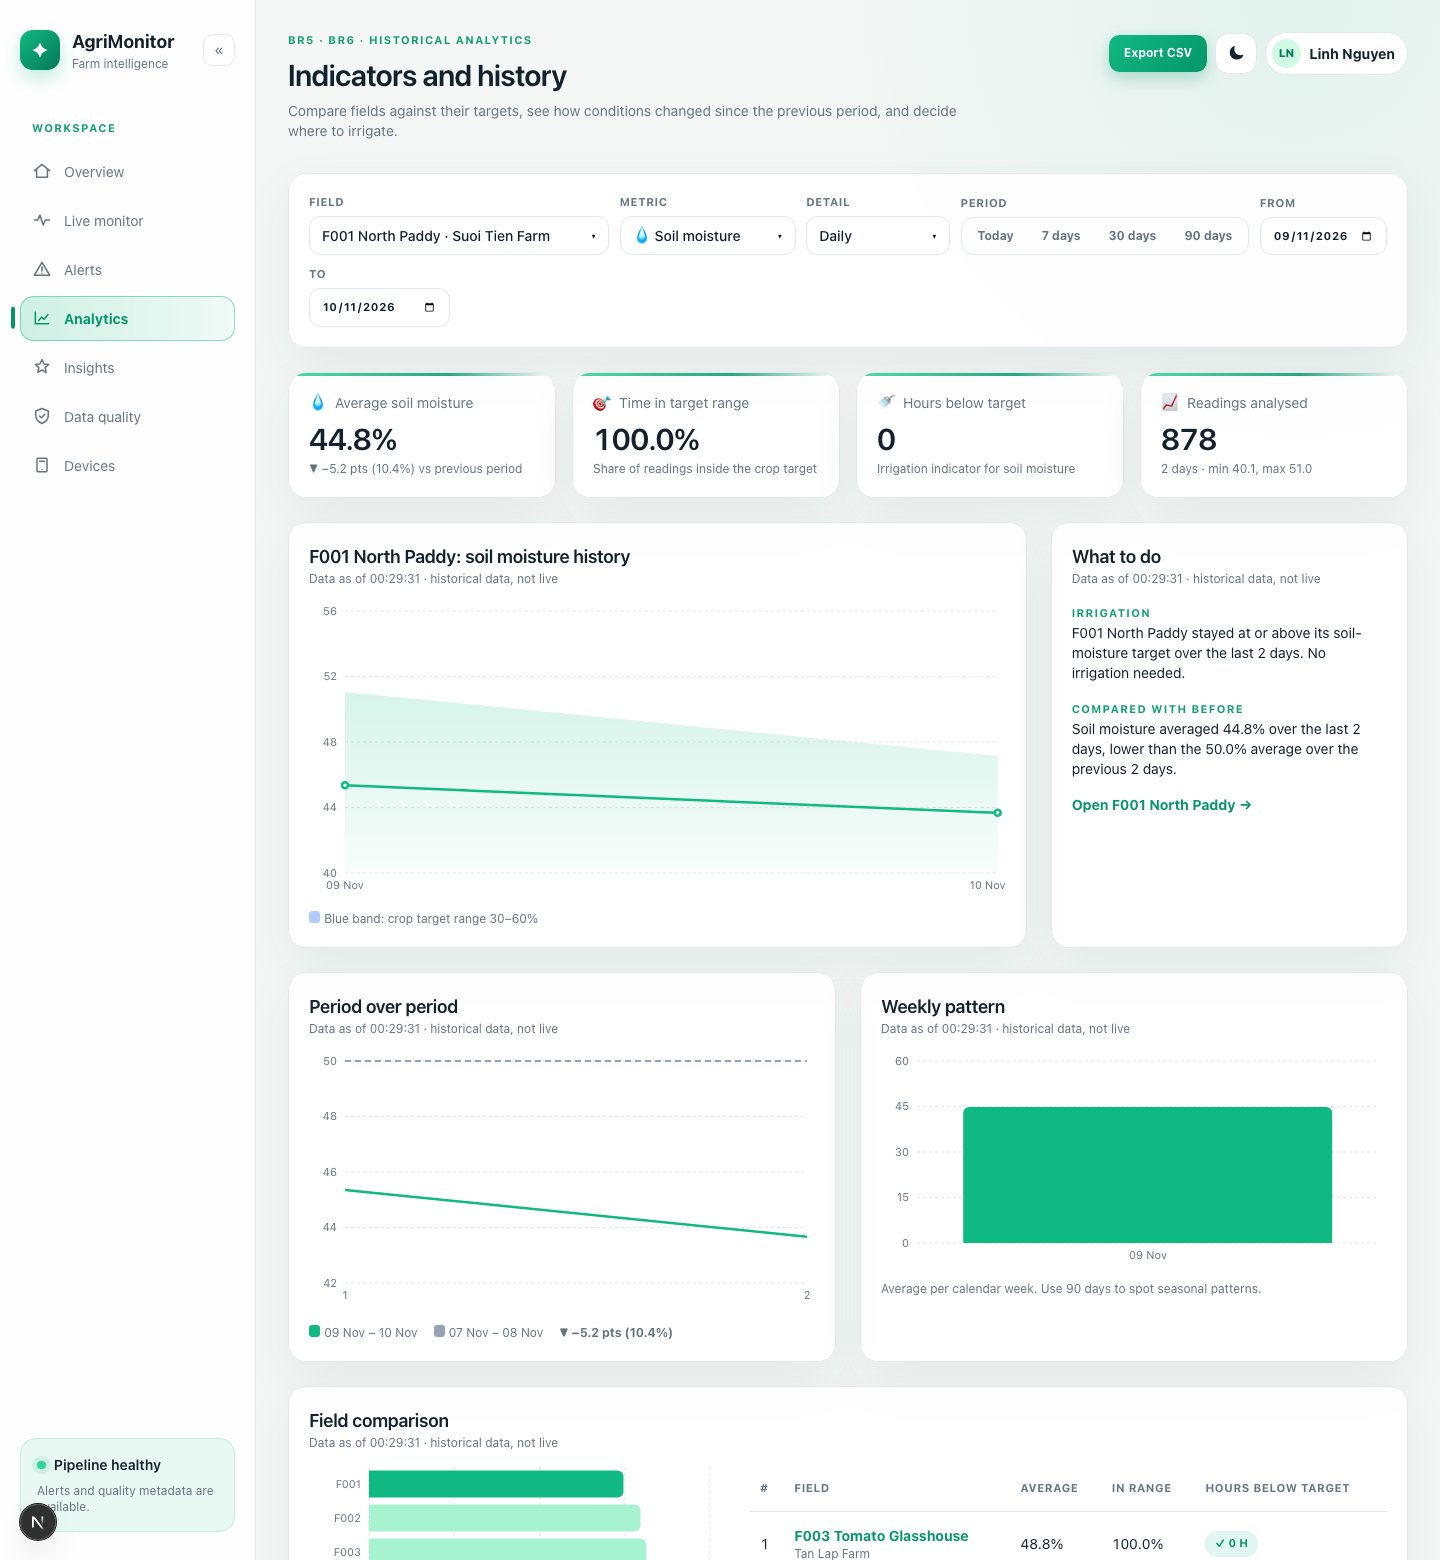
\includegraphics[width=0.95\linewidth]{analytics-period.png}
\caption{Trang Analytics: so sánh 9--10/11 với 7--8/11 của F001 (độ ẩm đất trung bình 44,8\% so với 50,0\%)}
\label{fig:4-br06-ui}
\end{figure}

\paragraph{Giới hạn của dữ liệu.} Bộ mô phỏng chỉ sinh dữ liệu trên một khoảng ngắn và thưa (nhiều ngày chỉ có một bản ghi), nên không có hai mùa vụ thật để so sánh và một số khoảng so sánh giai đoạn không có dữ liệu ở giai đoạn trước (giao diện hiển thị ``no data'' thay vì số 0). Tiêu chí về mùa vụ vì vậy chỉ chứng minh được \emph{cơ chế}: tổng hợp theo tuần và so sánh hai khoảng cùng độ dài. Báo cáo ghi nhận đây là một hạn chế (Mục~\ref{sec:5-discussion}). Nếu cần minh họa tốt hơn, có thể nạp trước một lịch sử mô phỏng dài hơn trước khi dựng gold, nhưng đó vẫn là dữ liệu mô phỏng chứ không phải mùa vụ thật.

\paragraph{Kịch bản minh họa.} Nhà phân tích chọn F001, so hai ngày gần nhất với hai ngày trước đó, và thấy độ ẩm đất trung bình giảm 5,2 điểm phần trăm. Họ chạy truy vấn time travel trên bảng \code{field\_indicators} tại snapshot đã ghi lúc xuất báo cáo và nhận lại đúng số liệu cũ, kể cả khi dữ liệu và khoảng mục tiêu đã đổi sau đó.


\section{So sánh với giải pháp thay thế}
\label{sec:5-comparison}
% Đầu vào của Khang cho Mục 5.5 (người phụ trách mục: Đạt): so sánh lớp lưu trữ và phục vụ phân tích.
\subsection{Lớp lưu trữ và phục vụ phân tích}
\label{sec:5-comparison-storage}

Mục~\ref{sec:4-alternative} đặt ra hai phương án thay thế; mục này đối chiếu chúng với giải pháp chính bằng số đo của Mục~\ref{sec:5-bench-khang}. Bảng~\ref{tab:5-compare-storage} so sánh Iceberg với Hive/Parquet thuần, Bảng~\ref{tab:5-compare-serving} so sánh hai đường phục vụ.

{\small
\begin{longtblr}[
  caption = {Iceberg và Hive/Parquet thuần: kết quả đo (Benchmark \#3, 1,2 triệu dòng, 240 commit)},
  label = {tab:5-compare-storage},
]{
  width = \linewidth,
  rowhead = 1,
  colspec = {X[2.4,l]X[2,l]X[2,l]X[1.6,l]}, rows = {abovesep=2pt, belowsep=2pt},
  hlines, vlines, row{1} = {font=\bfseries, bg=gray!20},
}
Tiêu chí & Iceberg (giải pháp chính) & Hive/Parquet & Bên thắng \\
Truy vấn 7 ngày, p50 & 135,6 ms & 76,7 ms (lọc theo cột phân vùng) & Hive \\
Cùng truy vấn nếu lọc theo \code{measured\_at} & 135,6 ms & 250,0 ms & Iceberg \\
Thời gian nạp mỗi commit & 3,2 s & 0,76 s & Hive \\
Phát lại một lô: dòng trùng & 0 & 5\,000 & Iceberg \\
Xem lại trạng thái cũ & có & không & Iceberg \\
Đổi tên cột có dữ liệu & 1\,200\,000 dòng còn đọc được & 0 dòng đọc được & Iceberg \\
Số tệp nhỏ & 720 & 720 & hòa \\
Độ phức tạp vận hành & cao hơn (dọn snapshot) & thấp & Hive \\
\end{longtblr}
}

Hive/Parquet nhanh hơn và rẻ hơn khi ghi, nhưng chỉ khi người viết truy vấn biết lọc theo cột phân vùng, và nó không có ba thứ mà đề tài cần: phát lại không sinh dòng trùng (BR3, BR4), xem lại quá khứ (BR6) và đổi schema không mất dữ liệu. Với dữ liệu nông nghiệp được tích lũy hằng ngày và phải tái tạo được báo cáo cũ, chi phí khoảng 4 lần ở thời gian commit (vẫn dưới 11\% chu kỳ trigger) là chấp nhận được. Nếu hệ thống chỉ cần ghi một lần và đọc, không phát lại, không đổi schema, Hive/Parquet đơn giản hơn là lựa chọn hợp lý.

\begin{table}[H]
\centering
\caption{Hai đường phục vụ và phương án chỉ dùng Cassandra (Benchmark \#2)}
\label{tab:5-compare-serving}
\small
\begin{tblr}{
  colspec = {X[2.4,l]X[2,l]X[2.4,l]}, rows = {abovesep=2pt, belowsep=2pt},
  hlines, vlines, row{1} = {font=\bfseries, bg=gray!20},
}
Tiêu chí & Cassandra & Trino trên Iceberg \\
Chuỗi 24 giờ (Q1), p50 ở 1 / 10 máy khách & 3,0 ms / 4,4 ms & 45,5 ms / 101,8 ms \\
Thông lượng Q1 ở 10 máy khách & 2\,046 truy vấn/giây & 89 truy vấn/giây \\
Lịch sử 30 ngày (Q2), p50 ở 1 máy khách & cần thêm một bảng và nạp lại dữ liệu & 42,2 ms từ bảng gold có sẵn \\
So sánh mọi thửa ruộng (Q3) & cần thêm một bảng & 45,1 ms từ bảng gold có sẵn \\
Giữ toàn bộ lịch sử thô để xử lý lại & không (TTL 24--48 giờ) & có (bronze) \\
\end{tblr}
\end{table}

Cassandra nhanh hơn Trino 15 đến 23 lần cho câu hỏi gần thời gian thực, và đây là lý do bảng điều khiển gần thời gian thực chỉ đọc Cassandra. Ngược lại, phương án chỉ dùng Cassandra buộc phải tạo một bảng cho mỗi câu hỏi phân tích mới và không giữ được dữ liệu thô để xử lý lại, hai thứ mà BR5 và BR6 đòi hỏi. Phương án chỉ dùng Trino cũng không đạt: p95 của tra cứu giá trị mới nhất ở 10 máy khách là 213 ms, cao hơn nhiều so với yêu cầu ``cỡ mười mili-giây''. Giải pháp hai đường phục vụ là phương án duy nhất đáp ứng cả hai nhóm yêu cầu, và cái giá là phải vận hành thêm một hệ thống.

\paragraph{Hiệu quả của việc gộp tệp.} Các con số của cả hai định dạng ở Bảng~\ref{tab:5-compare-storage} đều đo khi bảng còn 720 tệp nhỏ, chưa gộp. Với Iceberg, \code{rewrite\_data\_files} gộp còn 30 tệp trong 15 giây và làm truy vấn 7 ngày nhanh gấp 2,1 lần (Bảng~\ref{tab:5-bench-compaction}), nên khoảng cách với Hive ở truy vấn đó thu hẹp lại. Với Hive/Parquet, đề tài không đo việc gộp; muốn gộp phải tự viết lại các phân vùng.

% Đầu vào cho Mục 5.5 (người phụ trách mục: Đạt): so sánh lớp xử lý luồng (phương án C).
% Số liệu từ benchmark #1 (Nhân phụ trách), do Khang chạy.
\subsection{Lớp xử lý luồng: chu kỳ trigger và xử lý từng sự kiện}
\label{sec:5-comparison-trigger}

Bảng~\ref{tab:5-compare-trigger} đối chiếu giải pháp chính (micro-batch 30 giây) với phương án C của Mục~\ref{sec:4-alt-trigger}. Ba cột đầu là số đo của benchmark \#1 (Bảng~\ref{tab:5-bench-trigger}); cột cuối là phân tích, vì xử lý từng sự kiện kiểu Flink không được xây dựng.

\begin{table}[H]
\centering
\caption{Giải pháp chính và phương án C}
\label{tab:5-compare-trigger}
\small
\begin{tblr}{
  colspec = {X[2.2,l]X[1.2,l]X[1.4,l]X[1.2,l]X[1.8,l]}, rows = {abovesep=2pt, belowsep=2pt},
  hlines, vlines, row{1} = {font=\bfseries, bg=gray!20},
}
Tiêu chí & C: 10 s & Chính: 30 s & C: 60 s & C: từng sự kiện (phân tích) \\
Độ trễ đầu-cuối p95 & 16 s & 36 s & 64 s & dưới 1 s tới Cassandra \\
Độ trễ cảnh báo mất kết nối p50 & 17 s & 48 s & 95 s & cỡ thời gian im lặng cho phép (20 s), cần bộ hẹn giờ theo thiết bị \\
Tỷ lệ bận / CPU trung bình & 63\,\% / 31\,\% & 26\,\% / 13\,\% & 20\,\% / 12\,\% & chạy liên tục \\
Commit bronze mỗi giờ & 360 & 120 & 60 & vẫn phải gom lô trước khi ghi Iceberg \\
Đạt mục tiêu 90 s & có & có, dư nhiều & có & có \\
Công nghệ mới & không & không & không & Flink, nằm ngoài bảng quyết định \\
\end{tblr}
\end{table}

Phương án 10 giây cho độ trễ thấp hơn khoảng 2 lần nhưng làm tác vụ bận gần hai phần ba thời gian và tạo gấp 3 lần số tệp nhỏ; với chi phí cố định khoảng 6 giây mỗi lô, đây là cấu hình dễ tụt lại nhất khi tải tăng. Phương án 60 giây gần như không tiết kiệm thêm CPU so với 30 giây nhưng làm cảnh báo chậm gấp đôi. Xử lý từng sự kiện chỉ có lợi khi cần phản ứng trong vài giây, điều mà các quyết định nông nghiệp của đề tài (tưới, xử lý thiết bị hỏng) không đòi hỏi, trong khi phải đưa thêm một engine luồng và chuyển trạng thái cảnh báo vào engine đó. Giải pháp chính (30 giây) vì vậy được giữ nguyên.


\section{Thảo luận}
\label{sec:5-discussion}
% TODO
